



\documentclass[first=dgreen,second=purple,logo=yellowexc]{aaltoslides}
%\documentclass{aaltoslides} % DEFAULT
%\documentclass[first=purple,second=lgreen,logo=redque,normaltitle,nofoot]{aaltoslides} % SOME OPTION EXAMPLES





% input encode
\usepackage[utf8]{inputenc}


%\usepackage[T1]{fontenc}
%\usepackage{lastpage}
%\usepackage{multirow}
%\usepackage{colortbl}
%\usepackage{comment}
%\usepackage{bm}
%\usepackage{natbib}


% Lipsum package generates bullshit
%\usepackage{lipsum}

% Set the document languages
%\usepackage[finnish,swedish,english]{babel}

% nomenclature
%\usepackage[intoc]{nomencl}

% math
\usepackage{amsmath}

% bibliograph
%\usepackage{natbib}

% For algorithms
\usepackage{algorithm}
\usepackage{algorithmic}

% math font
\usepackage{amsfonts}

% theory
%\usepackage{amsthm}

% double bracket
\usepackage{stmaryrd}

% special math symbol
\usepackage{amssymb}

% use enumerate environment
%\usepackage{enumitem}

% use \url \hyperref, make reference clickable
\usepackage{hyperref}

% use lastpage to inde
\usepackage{lastpage}



%-------------------
%
% set
%
%-------------------
\newcommand{\Acal}{\mathcal{A}}
\newcommand{\Bcal}{\mathcal{B}}
\newcommand{\Ccal}{\mathcal{C}}
\newcommand{\Dcal}{\mathcal{D}}
\newcommand{\Ecal}{\mathcal{E}}
\newcommand{\Fcal}{\mathcal{F}}
\newcommand{\Gcal}{\mathcal{G}}
\newcommand{\Hcal}{\mathcal{H}}
\newcommand{\Ical}{\mathcal{I}}
\newcommand{\Jcal}{\mathcal{J}}
\newcommand{\Kcal}{\mathcal{K}}
\newcommand{\Lcal}{\mathcal{L}}
\newcommand{\Mcal}{\mathcal{M}}
\newcommand{\Ncal}{\mathcal{N}}
\newcommand{\Ocal}{\mathcal{O}}
\newcommand{\Pcal}{\mathcal{P}}
\newcommand{\Qcal}{\mathcal{Q}}
\newcommand{\Rcal}{\mathcal{R}}
\newcommand{\Scal}{\mathcal{S}}
\newcommand{\Tcal}{\mathcal{T}}
\newcommand{\Ucal}{\mathcal{U}}
\newcommand{\Vcal}{\mathcal{V}}
\newcommand{\Wcal}{\mathcal{W}}
\newcommand{\Xcal}{\mathcal{X}}
\newcommand{\Ycal}{\mathcal{Y}}
\newcommand{\Zcal}{\mathcal{Z}}

\newcommand{\RR}{\mathbb{R}}
\newcommand{\ZZ}{\mathbb{Z}}

%-------------------
%
% vector
%
%-------------------
\newcommand{\va}{\mathbf {a}}
\newcommand{\vb}{\mathbf {b}}
\newcommand{\vc}{\mathbf {c}}
\newcommand{\vd}{\mathbf {d}}
\newcommand{\ve}{\mathbf {e}}
\newcommand{\vf}{\mathbf {f}}
\newcommand{\vg}{\mathbf {g}}
\newcommand{\vh}{\mathbf {h}}
\newcommand{\vi}{\mathbf {i}}
\newcommand{\vj}{\mathbf {j}}
\newcommand{\vk}{\mathbf {k}}
\newcommand{\vl}{\mathbf {l}}
\newcommand{\vm}{\mathbf {m}}
\newcommand{\vn}{\mathbf {n}}
\newcommand{\vo}{\mathbf {o}}
\newcommand{\vp}{\mathbf {p}}
\newcommand{\vq}{\mathbf {q}}
\newcommand{\vr}{\mathbf {r}}
\newcommand{\vs}{\mathbf {s}}
\newcommand{\vt}{\mathbf {t}}
\newcommand{\vu}{\mathbf {u}}
\newcommand{\vv}{\mathbf {v}}
\newcommand{\vw}{\mathbf {w}}
\newcommand{\vx}{\mathbf {x}}
\newcommand{\vy}{\mathbf {y}}
\newcommand{\vz}{\mathbf {z}}
\newcommand{\vmu}{\mathbf {\mu}}
\newcommand{\valpha}{\mathbf {\alpha}}
\newcommand{\vlambda}{\mathbf {\lambda}}
\newcommand{\vAlpha}{\mathbf {\Alpha}}
\newcommand{\vbeta}{\mathbf {\beta}}
\newcommand{\vBeta}{\mathbf {\Beta}}
\newcommand{\vgamma}{\mathbf {\gamma}}
\newcommand{\vGamma}{\mathbf {\Gamma}}
\newcommand{\vdelta}{\mathbf {\dalta}}
\newcommand{\vDelta}{\mathbf {\Dalta}}
\newcommand{\vone}{\mathbf {1}}
\newcommand{\vzero}{\mathbf {0}}
\newcommand{\vell}{\mathbf {\ell}}
\newcommand{\vxi}{\mathbf{\xi}}
\newcommand{\vphi}{\mathbf{\phi}}
\newcommand{\vPhi}{\mathbf{\Phi}}

%-------------------
%
% math operation
%
%-------------------
\newcommand{\argmax}{\textbf{argmax}}
\newcommand{\argmin}{\textbf{argmin}}
\newcommand{\sign}{\textbf{sign}}
\newcommand{\maximize}{\textbf{max}}
\newcommand{\minimize}{\textbf{min}}
\newcommand{\argkmax}{\textbf{argkmax}}
\newcommand{\argkmin}{\textbf{argkmin}}
\newcommand{\kmaximize}{\textbf{kmax}}
\newcommand{\kminimize}{\textbf{kmin}}
\newcommand{\st}{\textbf{s.t.}}
\newcommand{\set}[1]{\{ #1 \}}
%\newcommand{\ind}[1]{{\llbracket #1 \rrbracket}}
\newcommand{\ind}[1]{\mathbf{1}_{\{#1\}}}
\newcommand{\norm}[1]{\left|\left| #1 \right|\right|}
\newcommand{\ip}[2]{\langle #1, #2 \rangle}
\newcommand{\var}{\textbf{Var}}
\newcommand{\E}{\textbf{E}}
\newcommand{\exponential}[1]{e^{ #1 }}


\newcommand{\Gva}{G_{\va}}
%-------------------
%
% writings
%
%-------------------
\newcommand{\eqdef}{\overset{{\rm \mbox{\tiny def}}}{=}}
\newcommand{\sbf}[1]{\boldsymbol{#1}}
\newcommand{\mbf}[1]{\mathbf{#1}} 
\newcommand{\etal}{{\em et al.}}

\newcommand{\svmstruct}{{\sc ssvm}}
\newcommand{\mmmn}{{\sc m$^3$n}}
\newcommand{\svm}{{\sc svm}}
\newcommand{\mmcrf}{{\sc mmcrf}}
\newcommand{\smo}{{\sc smo}}
\newcommand{\crf}{{\sc crf}}
\newcommand{\nphard}{$\Ncal\Pcal$-hard}
\newcommand{\nphardness}{$\Ncal\Pcal$-hardness}
\newcommand{\iis}{{\sc iis}}
\newcommand{\memm}{{\sc memm}}
\newcommand{\lr}{{\sc lr}}
\newcommand{\svmlight}{{\sc svmlight}}
\newcommand{\libsvm}{{\sc libsvm}}
\newcommand{\svmcascade}{{\sc svmcascade}}
\newcommand{\adaboost}{{\sc adaboost}}
\newcommand{\adaboostmh}{{\sc adaboost.mh}}
\newcommand{\bagging}{{\sc bagging}}
\newcommand{\vrtree}{{\sc vr-tree}}
\newcommand{\deepboosting}{{\sc deepboosting}}
\newcommand{\loo}{{\sc loo}}
\newcommand{\mtl}{{\sc mtl}}
\newcommand{\sdp}{{\sc sdp}}
\newcommand{\iqp}{{\sc iqp}}
\newcommand{\qp}{{\sc qp}}
\newcommand{\daggraph}{{\sc dag}}
\newcommand{\lp}{{\sc lp}}

\newcommand{\hatf}{{\hat{f}}}
\newcommand{\p}{\sc p}
\newcommand{\n}{\sc n}
\newcommand{\pp}{\sc pp}
\newcommand{\pn}{\sc pn}
\newcommand{\nn}{\sc nn}
\newcommand{\maxcut}{{\sc max-cut}}
\newcommand{\greedy}{{\sc greedy}}
\newcommand{\kernelcascade}{{\sc kernel cascade}}
\newcommand{\netrate}{{\sc netrate}}
\newcommand{\netinf}{{\sc netinf}}
\newcommand{\spin}{{\sc spin}}
\newcommand{\vI}{\mathbf{I}}
\newcommand{\tp}{^{\intercal}}
\newcommand{\mve}{{\sc mve}}
\newcommand{\amm}{{\sc amm}}
\newcommand{\mam}{{\sc mam}}
\newcommand{\rta}{{\sc rta}}
\newcommand{\lasso}{{\sc lasso}}
\newcommand{\mle}{{\sc mle}}
\newcommand{\map}{{\sc map}}
\newcommand{\rbf}{{\sc rbf}}
\newcommand{\mlknn}{{\sc ml-knn}}
\newcommand{\knn}{{\sc knn}}
\newcommand{\iblr}{{\sc iblr}}
\newcommand{\cc}{{\sc cc}}
\newcommand{\pcc}{{\sc pcc}}
\newcommand{\ecc}{{\sc ecc}}
\newcommand{\br}{{\sc br}}
\newcommand{\corrlog}{{\sc corrlog}}
\newcommand{\ilgs}{{\sc ilgs}}
\newcommand{\ilrs}{{\sc ilrs}}
\newcommand{\cpp}{{\sc c}}
\newcommand{\matlab}{{\sc matlab}}
\newcommand{\openmp}{{\sc openmp}}
\newcommand{\python}{{\sc python}}
\newcommand{\cvx}{{\sc cvx}}
\newcommand{\lda}{{\sc lda}}
\newcommand{\kkt}{{\sc k.k.t}}
\newcommand{\lbp}{{\sc lbp}}
\newcommand{\anova}{{\sc anova}}

\renewcommand{\algorithmicrequire}{\textbf{Input:}}
\renewcommand{\algorithmicensure}{\textbf{Output:}}



\newcommand{\Upsilonb}{\pmb \Upsilon}
\newcommand{\phib}{\pmb \phi}
\newcommand{\psib}{\pmb \psi}
\newcommand{\varphib}{\pmb \varphi}
\newcommand{\phibh}{\hat\phib}
\newcommand{\psibh}{\hat \psib}
\newcommand{\vYcal}{\pmb \Ycal}
\newcommand{\vXcal}{\pmb \Xcal}
\newcommand{\vFcal}{\pmb \Fcal}
%-------------------
%
% others
%
%-------------------




%\newtheorem{definition}{Definition}
%\newtheorem{theory}{Theory}
%\newtheorem{lemma}{Lemma}

















\title{Structured output prediction for multilabel classification}
\author{Hongyu Su}



\institute[ICS]{
Helsinki Institute for Information Technology HIIT\\
Department of Computer Science, Aalto University
}

\aaltofootertext{Structured output prediction}{\today}{\arabic{page}\ }


\date{ \today} %\date{Version 1.0, \today}

\iffalse
\AtBeginSection[]
{
  \begin{frame}<beamer>{Outline}
    \tableofcontents[currentsection,subsection]
  \end{frame}
}
\fi




%--------------------------------
%
% document
%
%--------------------------------

\begin{document}

\aaltotitleframe
\footnotesize

%
\begin{frame}{}
	\begin{center}
		The update-to-date version of this slide is available from \href{https://github.com/hongyusu/Posters_and_Presentations/raw/master/Presentations/Seminar/example.pdf}{my GitHub page}.
	\end{center}
\end{frame}

\begin{frame}{About me}
	\begin{center}
		Take a look at \href{http://hongyusu.github.io}{my homepage} and \href{http://hongyusu.github.io/pages.html}{my technical blog}.
	\end{center}
\end{frame}

%
\begin{frame}{Multilabel classification}
	\begin{itemize}\footnotesize
		\item It is an important research field in machine learning.
		\item Input variable $\vx\in\vXcal$ lives in some input space $\vXcal$.
		\item Output variable $\vy=(y_1,\cdots,y_l)\in\vYcal$ is a vector of $\ell$ binary variables $y_j\in\{+1,-1\}$.
		\item $\vy$ is called {\em multilabel}, $y_j$ is called {\em microlabel}.
		\item Output space $\vYcal$ is composed by a tensor product of $\ell$ sets
		\begin{align*}
			\vYcal=\Ycal_1\times\cdots\times\Ycal_{\ell},\,\Ycal_i=\{+1,-1\}.
		\end{align*}
		\item For example, in document classification, a document $\vx$ could be tagged with {\blue``news'' ``movie'' ``science''} but not {``sports'' ``politics'' ``finance''}.
		\begin{align*}
\vy=(\underbrace{+1}_{\blue\text{news}},\underbrace{+1}_{\blue\text{movie}},\underbrace{-1}_{\text{sports}},\underbrace{-1}_{\text{politics}},\underbrace{-1}_{\text{finance}},\underbrace{+1}_{\blue\text{science}},\underbrace{-1}_{\text{art}}).
		\end{align*}\footnotesize
		\item The goal is to find a mapping function $f\in\Hcal$ that predicts the best values of an output $\vy$ given an input $\vx$, $f:\vXcal\rightarrow\vYcal$.
	\end{itemize}
\end{frame}

%
\begin{frame}{Concerns}
	\begin{itemize}\footnotesize
		\item Dimension of the search space: exponential in the number of microlabels.
		\begin{align*}
			\vYcal=\Ycal_1\times\cdots\times\Ycal_{\ell},\,\Ycal_i=\{+1,-1\}\quad|\vYcal| = 2^{\ell}.
		\end{align*}
		\item The dependency of microlabels needs to be exploited.
		\begin{itemize}\footnotesize
			\item If a document is tagged with ``movie'', then it is more likely to be in the category of ``art'' than ``science''.
		\end{itemize}
	\end{itemize}
\end{frame}

%
\begin{frame}{Applications}
	\begin{itemize}\footnotesize
		\item Social network, information can spread through multiple users. 
		\begin{tabular}{p{3cm}p{10cm}} 
	    \multirow{2}{*}{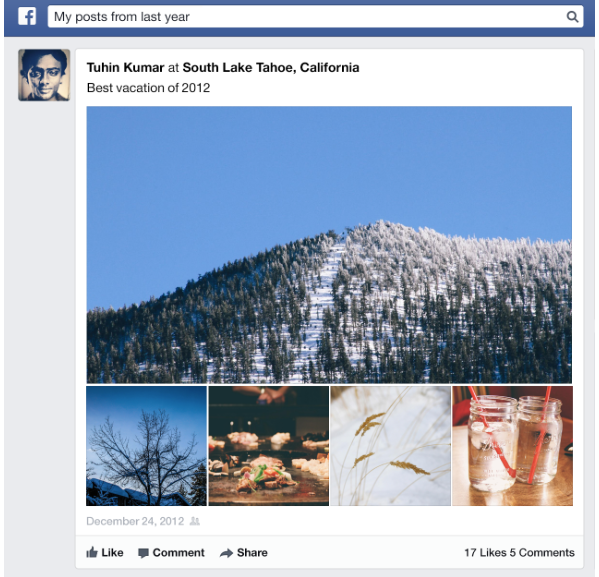
\includegraphics[scale = 0.06]{./figures/facebookvideo.png}} & \\
		& $\vy=(\underbrace{+1}_{\text{Ted}},\underbrace{-1}_{\text{Alice}},\underbrace{+1}_{\text{David}},\underbrace{-1}_{\text{Mark}},\underbrace{+1}_{\text{Alex}},\underbrace{-1}_{\text{Zoe}},\underbrace{-1}_{\text{Frank}})$\\
	    \end{tabular}
		\item Image annotation, an image can associate with multiple tags.
		\begin{tabular}{p{3cm}p{10cm}}
        \multirow{2}{*}{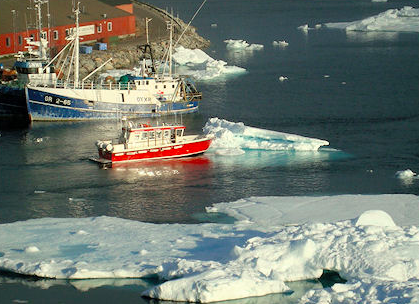
\includegraphics[scale = 0.11]{./figures/boatsea.png}} & \\
		& $\vy=(\underbrace{+1}_{\text{boat}},\underbrace{+1}_{\text{sea}},\underbrace{-1}_{\text{sun}},\underbrace{-1}_{\text{beach}},\underbrace{-1}_{\text{people}},\underbrace{+1}_{\text{ice}},\underbrace{+1}_{\text{land}})$\\
        \end{tabular}
		\item Document classification, an article can be assigned to multiple categories.
		\begin{tabular}{p{3cm}p{10cm}} 
        \multirow{2}{*}{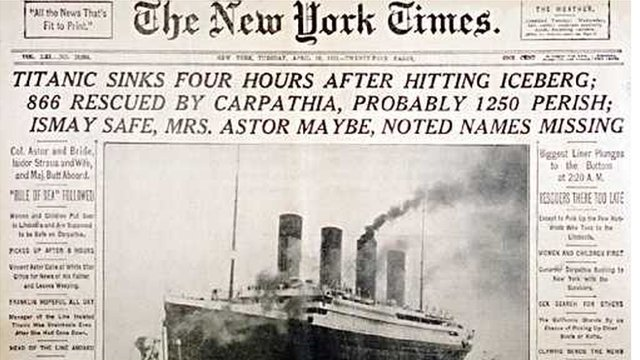
\includegraphics[scale = 0.11]{./figures/titanic.jpg}} & \\
		& $\vy=(\underbrace{+1}_{\text{news}},\underbrace{+1}_{\text{economics}},\underbrace{-1}_{\text{sports}},\underbrace{-1}_{\text{politics}},\underbrace{-1}_{\text{movie}},\underbrace{-1}_{\text{science}},\underbrace{-1}_{\text{art}})$\\
        \end{tabular}
		\item Drug discovery, a drug can be effective for multiple symptoms.
		\begin{tabular}{p{3cm}p{10cm}} 
        \multirow{2}{*}{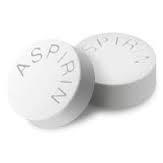
\includegraphics[scale = 0.25]{./figures/aspirin.jpg}} & \\
		& $\vy=(\underbrace{+1}_{\text{heart}},\underbrace{+1}_{\text{stroke}},\underbrace{+1}_{\text{blood}},\underbrace{+1}_{\text{fever}},\underbrace{-1}_{\text{digest}},\underbrace{-1}_{\text{liver}},\underbrace{+1}_{\text{swelling}})$\\
        \end{tabular}
	\end{itemize}
\end{frame}

%
\begin{frame}{Flat multilabel classification}
	\begin{itemize}\footnotesize
		\item The scheme is proposed in \cite{Tsoumakas10mining}
		\item The output variable $\vy$ is assumed to be a flat vector.
		\item Problem transformation
		\begin{itemize}\footnotesize
			\item Model the problem as a collection of single-label classification problems and solve each problem independently.
			\item E.g., \mlknn\ \cite{Zhang07mlknn}, \cc\ \cite{Read11classifier}, \iblr\ \cite{Cheng09combining}.
		\end{itemize}
		\item Algorithm adaptation 
		\begin{itemize}\footnotesize
			\item Adapt single-label classification models to multilabel classification problems.
			\item E.g., \corrlog\ \cite{Bian12corrlog}, \mtl\ \cite{Argyriou08convex}, \adaboostmh\ \cite{Schapire99improved,Esuli2008boosting}.
		\end{itemize}
		\item These approaches does not model the dependency structure of microlabels explicitly.
	\end{itemize}
\end{frame}

%
\begin{frame}{Structured output prediction}
	\begin{itemize}\footnotesize
		\item Model the dependency structure with an {\em output graph} defined on microlabels.
		\item The categorization is proposed in \cite{Su2014Multilabel}.
		\item Hierarchical classification
		\begin{itemize}\footnotesize
			\item The output graph is a rooted tree defining different levels of granularities.
			\item For example, \svmstruct\ \cite{THJA04,TJTA05}.
		\end{itemize}
		\item Graph labeling
		\begin{itemize}\footnotesize
			\item The output graph takes a more general form (e.g., a tree, a chain).
			\item For example, \crf\ \cite{lafferty01,taskar02}, \mmmn\ \cite{Taskar04max}, \mmcrf\ \cite{Rousu07, su10structured}, \spin\ \cite{su14structured}.
		\end{itemize}
		\item These approaches assume the output graph is known {\em apriori}.
	\end{itemize}
\end{frame}

%
\begin{frame}{Contributions}
	\begin{itemize}\footnotesize
		\item Structured output prediction models when the output graph is known.
		\begin{itemize}\footnotesize
			\item \spin\ for network influence prediction \cite{su14structured}.
			\item \mmcrf\ to work with general output graph structures \cite{su10structured}.
		\end{itemize}
		\item Structured output prediction models working with unknown output graph.
		\begin{itemize}\footnotesize
			\item \mve\ to combine multiple structured output predictors by ensemble \cite{su11mutitask}.
			\item \amm\ and \mam\ to aggregate the inference results from multiple structured output predictors \cite{su2013multilabelacml,su15multilabel}.
			\item \rta\ to perform joint learning and inference over a collection of random spanning tree predictors \cite{su14multilabelnips}.
		\end{itemize}
		\item Codes for developed models are available from \href{http://hongyusu.github.io}{http://hongyusu.github.io}.
	\end{itemize}
\end{frame}


%
\begin{frame}{Outline}
	\begin{itemize}\footnotesize
		\item Preliminaries
		\item Structured output prediction
		\begin{itemize}\footnotesize
			\item Undirected graph structure
			\item \daggraph\ structure
			\item unknown structure
		\end{itemize}
		\item Experimental evaluations
		\item Conclusion and future work
	\end{itemize}
\end{frame}

%
\begin{frame}{Preliminaries}
	\begin{itemize}\footnotesize
		\item Training examples come in pairs $(\vx,\vy)\in\vXcal\times\vYcal$.
		\item $\vx\in\vXcal$ is an arbitrary input space.
		\item $\vYcal$ is an output space of a collection of $\ell$-dimensional {\em multilabels}.
		\begin{align*}\footnotesize
			\vy=(y_1,\cdots,y_{\ell})\in\vYcal.
		\end{align*}
		\item $y_i$ is a {\em microlabel} and $y_i\in\{1,\cdots,r_i\}, r_i\in\ZZ$.
		\item For example, multilabel binary classification $y_i\in\{-1,+1\}$.
		\item We are given a set of $m$ training examples $\{(\vx_i,\vy_i)\}_{i=1}^m$.
		%\item An arbitrary pair $(\vx_i,\vy),\,\vy_\in\vYcal$ is called pseudo-example.
		\item Each example $(\vx,\vy)$ is mapped into a joint feature space $\phib(\vx,\vy)$.
		\item $\vw$ is the weight vector in the joint feature space.
		\item Define a linear score function $F(\vw,\vx,\vy) = \ip{\vw}{\phib(\vx,\vy)}$.
		\item $\vw$ makes sure example $\vx$ with correct multilabel $\vy$ achieves higher score than with any other incorrect multilabel $\vy'\in\vYcal$.
	\end{itemize}
\end{frame}

\begin{frame}{Inference problem}
	\begin{itemize}
		\item The prediction $\vy_{\vw}(\vx)$ of an input $\vx$ is the multilabel $\vy$ that maximizes the score function 
		\begin{align}\footnotesize
			\vy_{\vw}(\vx) = \underset{\vy\in\vYcal}{\argmax}\,\ip{\vw}{\phib(\vx,\vy)}. \label{inference}
		\end{align}
		\item Search space is exponential in size, $|\vYcal|=2^{\ell}$.
		\item (\ref{inference}) is called {\em inference} problem which is \nphard\ for most output feature maps.
		\item We aim at using an output feature map in which the inference can be solved with a polynomial algorithm, e.g., dynamic programming.
	\end{itemize}
\end{frame}

%
\begin{frame}{Input-output feature maps}
	\begin{itemize}\footnotesize
		\item We assume that the joint feature map $\phib$ is a potential function on a Markov network (undirected graph) $G=(E,V)$.
		\item A vertex $v_i\in V$ corresponds to a microlabel $y_i$, an edge $(v_i,v_j)\in E$ corresponds to the pairwise correlation of the microlabel $y_i$ and $y_j$.
		\item $G$ models potential pairwise correlations and is given {\em apriori}.
		\begin{center}
			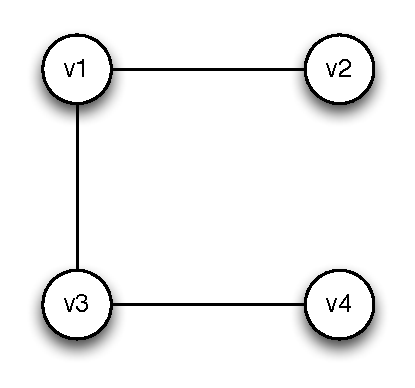
\includegraphics[scale=0.3]{./figures/outputgraph.pdf}
		\end{center}
		\item $\varphib(\vx)\in\RR^d$ is the input feature map, e.g., bag-of-words of a document.
		\item $\psib(\vy)\in\RR^{4|E|}$ is the output feature map which maps the multilabel $\vy$ into a collection of edges and labels
		\begin{align*}\footnotesize
			\varphib(\vy) = (u_{e})_{e\in E},u_e\in\{-1,+1\}^2.
		\end{align*}
	\end{itemize}
\end{frame}

%
\begin{frame}{An example of output feature map}
	\begin{itemize}\footnotesize
		\item Markov network (undirected graph) $G=(E,V)$
		\begin{center}
			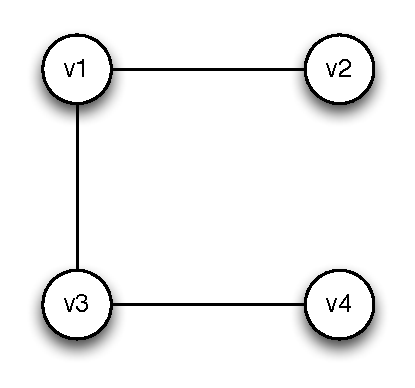
\includegraphics[scale=0.3]{./figures/outputgraph.pdf}
		\end{center}
		\item Multilabel $\vy$
		\begin{align*}
			\vy&=(y_1,y_2,y_3,y_4)=(+1,-1,+1,+1)
		\end{align*}
		\item Output feature map $\psib(\vy)$
		\begin{align*}
			\psib(\vy) &= ( \underbrace{\underbrace{0}_{--}, \underbrace{0}_{-+}, \underbrace{1}_{+-}, \underbrace{0}_{++},}_{(v_1,v_3)} 
			\underbrace{\underbrace{0}_{--}, \underbrace{0}_{-+}, \underbrace{0}_{+-}, \underbrace{1}_{++},}_{(v_1,v_2)}
			\underbrace{\underbrace{0}_{--}, \underbrace{0}_{-+}, \underbrace{0}_{+-}, \underbrace{1}_{++}}_{(v_3,v_4)})
		\end{align*}
	\end{itemize}
\end{frame}

%
\begin{frame}{Joint feature map}
	\begin{itemize}\footnotesize
		\item The joint feature is the Kronecker product of $\varphib(\vx)$ and $\psib(\vy)$
		\begin{align*}\footnotesize
			\phib(\vx,\vy) = (\phib_e(\vx,\vy))_{e\in E}=(\varphib(\vx)\otimes\psib_e(\vy_e))_{e\in E}.
		\end{align*}
		\begin{center}
			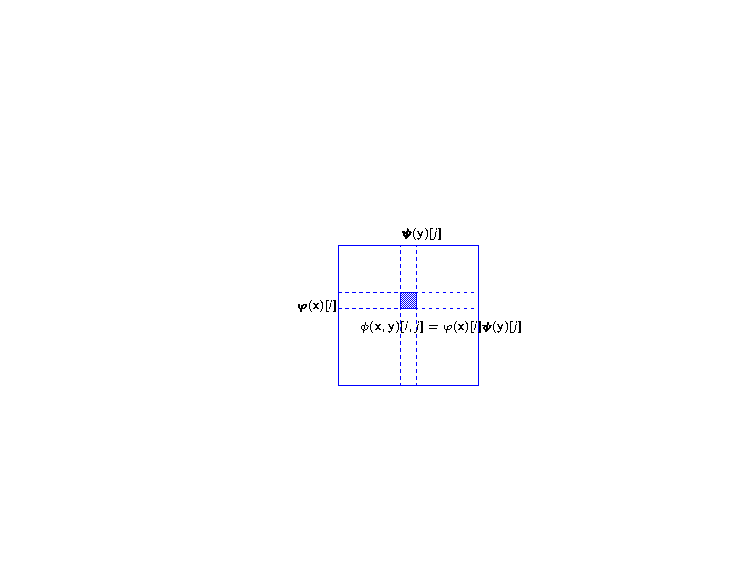
\includegraphics[scale = 1]{./figures/tensor_label.pdf}
		\end{center}
		\item The score function can be factorized by the output graph $G$
		\begin{align*}
			F(\vw,\vx,\vy) = \ip{\vw}{\phib(\vx,\vy)} = \sum_{e\in E}\ip{\vw_e}{\phib_e(\vx,\vy_e)}.
		\end{align*}
	\end{itemize}
\end{frame}

%
\begin{frame}{Optimization problem}
	\begin{itemize}\footnotesize
		\item To learn parameter $\vw$, we aim to maximize the magin between correct pair $(\vx_i,\vy_i)$ and all the other incorrect pairs $(\vx_i,\vy),\vy\in\vYcal/\vy_i$ in the joint feature space $\phib$.
		\begin{center}
			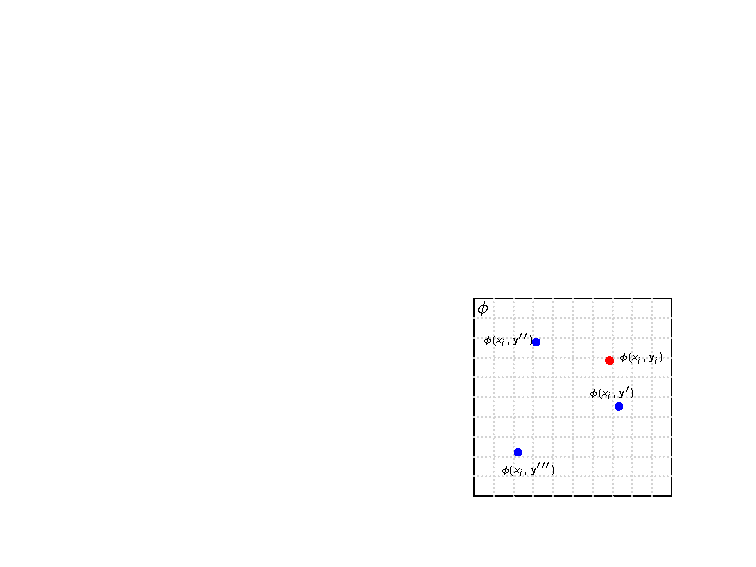
\includegraphics[scale = 0.6]{./figures/jointfeaturespace.pdf}
		\end{center}
		\item The model is max-margin conditional random field \mmcrf\ \cite{Rousu07, su10structured}.
		\item The primal optimization problem is defined as
		\begin{align}
			\underset{\vw,\xi_k}{\minimize} & \quad \frac{1}{2}\norm{\vw}^2 + C\sum_{k=1}^{m}\xi_k \label{primalmmcrf}\\
			\st & \quad \ip{\vw}{\phib(\vx_k,\vy_k)} - \ip{\vw}{\phib(\vx_k,\vy)}  \geq \ell(\vy_k,\vy) -  \xi_k, \nonumber\\
			& \quad \xi_k\ge0\, , \forall\ \vy\in\vYcal, k \in \set{1,\dots,m}.\nonumber
		\end{align}
		\item $\ell(\vy,\vy_k)$ scales the margin according to the multilabel $\vy$.
		%\item (\ref{primalmmcrf}) is difficult as the number of the constraints is $m\times|\vYcal|$.
	\end{itemize}
\end{frame}

%
\begin{frame}{Marginal-dual optimization}
	\begin{itemize}\footnotesize
		\item (\ref{primalmmcrf}) is difficult as the number of the constraints is $m\times|\vYcal|$.
		\item The dual optimization problem is defined as
		\begin{align}
			\underset{\valpha\ge0}{\maximize} & \quad \valpha^{\tp}\vell - \frac{1}{2}\valpha^{\tp}K\valpha\label{mmcrfdual}\\
			\st & \quad \sum_{\vy\in\vYcal}\alpha(k,\vy)\le C, \, \forall k\in\{1,\cdots,m\}\nonumber.
		\end{align}
		\item (\ref{mmcrfdual}) is also challenging due to the exponential number of dual variables.
		\item We use edge marginals to replace the dual variables \cite{Taskar04max}
		\begin{align*}
			\mu(k,e,u_e) = \sum_{\vy}\ind{\psib_e(\vy)=u_e}\alpha(k,\vy). 
		\end{align*}
		\item The margin-dual optimization problem is 
		\begin{align}
			\underset{\vmu\in\Mcal}{\maximize} & \quad \vmu^{\tp}\ell - \frac{1}{2}\vmu^{\tp}K\vmu. \label{mmcrfmarginaldual}
		\end{align}
		\item The number of marginal-dual variables is $m\times4|E|$.
	\end{itemize}
\end{frame}

%
\begin{frame}{Conditional gradient optimization}
	\begin{itemize}\footnotesize
		\item (\ref{mmcrfmarginaldual}) is optimized by conditional gradient decent.
		\item In each iteration it optimizes $\mu_k$ that corresponds to a single example while keeps others ($\mu_j,j\neq k$) fixed 
		\begin{align*}
			\underset{\vmu_k\in\Mcal}{\maximize} & \quad \vmu_k^{\tp}\ell_k - \frac{1}{2}\sum_{j}\vmu_k^{\tp}K\vmu_j, \, \forall k.
		\end{align*}
		\item Current gradient of $\mu_k$ is given by $g_i = \ell_{i}-\sum_{j}K\mu_j$.
		\item Compute the maximal feasible solution $\mu_k^*$ as an update direction
		\begin{align}
			\mu_k^* = \underset{\mu_k\in\Mcal}{\argmax} \, \mu_k^{\tp}g_k = \underset{\mu_k\in\Mcal}{\argmax} \, \sum_e\mu(k,e)^{\tp}g(k,e). \label{inferencemarginaldual}
		\end{align}
		\item (\ref{inferencemarginaldual}) is an instantiation of \map\ problem 
		\begin{tabular}{|c|c|c|}
			\hline
			\footnotesize
			 Output graph & Inference problem & Inference algorithm \\ \hline
			 Tree & Polynomial & DP \cite{Rousu07}  \\
			 Graph & \nphard & LBP \cite{su10structured}  \\ \hline
		\end{tabular}
		\item Perform the update via exact line search $\mu_k \leftarrow \mu_k + \tau(\mu_k^*-\mu_k)$.
	\end{itemize}
\end{frame}

%
\begin{frame}{Exact line search}
	\begin{itemize}
		\item Line search gives the optimal feasible solution as a stationary point ($\tau$)
		\begin{align}
			\underset{\tau}{\maximize} &\quad g(\vmu_k + \tau\Delta\vmu_{k})\label{tree_line_search}\\
			\st &\quad 0\le\tau\le1.\nonumber
		\end{align}
		\item $\tau=0$ corresponds to no update.
		\item Feasible maximum update is achieved at $\tau=1$. 
		\item The cost of computing (\ref{tree_line_search}) is significantly smaller than the cost of computing (\ref{inferencemarginaldual}).
	\end{itemize}
\end{frame}

%
\begin{frame}{Compute duality gap}
	\begin{itemize}\footnotesize
		\item We use duality gap to measure the progress of the optimization.
		\item Primal and marginal-dual objective functions
		\begin{align*}\footnotesize
			f(\vw) &= \frac{1}{2}||\vw||^2 + C\sum_{k=1}^m\left(\ell_k-\ip{\vw}{\Delta\phib(\vx_k,\vy_k)}\right)\\
			g(\vmu) &= \sum_{k=1}^m\mu_k\ell_k - \frac{1}{2}\sum_{k=1}^m\sum_{j=1}^m\mu_kK^{\Delta\phib}(\vx_k,\vy_k;\vx_j,\vy_j)\mu_j
		\end{align*}
		\item $\underset{\vmu}{\maximize}\,g(\vmu)\le \underset{\vw}{\minimize}\,f(\vw)$, gap is minimized at optimal.
		\item Duality gap at $\vmu^t$
		\begin{align*}\footnotesize
			f(\vw^t) - g(\vmu^t) &= C\left(\vell-K^{\Delta\phib}\vmu^t\right) - \vmu^t\left(\vell-K^{\Delta\phib}\vmu^t\right)\\
			&= C\tp \nabla g(\vmu^t) -{\vmu^t} \tp \nabla g(\vmu^t)
		\end{align*}
	\end{itemize}
		\begin{enumerate}\footnotesize
			\item Estimate the marginal-dual objective by linear approximation $\nabla g(\vmu^t)$.
			\item Marginal-dual objective value at $\vmu^t$ is computed by ${\vmu^t} \tp \nabla g(\vmu^t)$.
			\item Primal objective value is estimate by $C\tp \nabla g(\vmu^t)$.
		\end{enumerate}
\end{frame}

%
\begin{frame}{Output graph is directed}{Predicting network response}
	\only<1>{A twitter (follower-ship) network consists of five users. 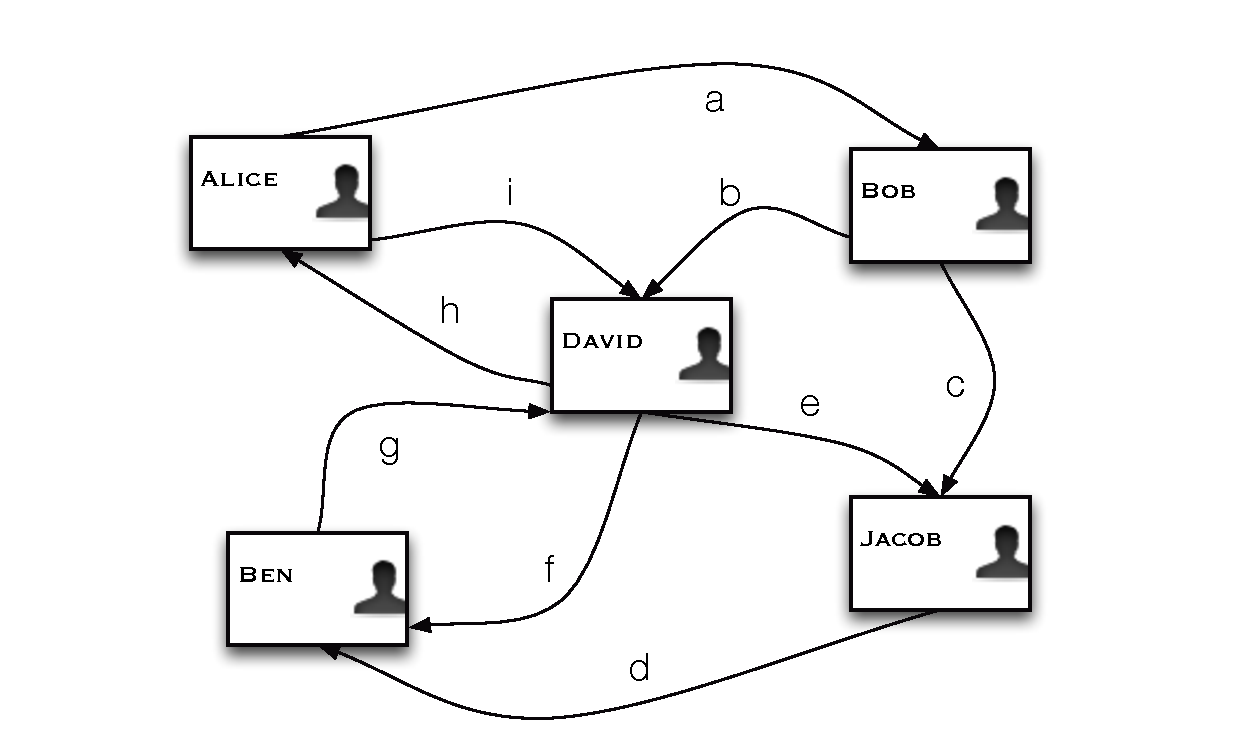
\includegraphics[scale=0.5]{./figures/motivation_1.pdf}}
	\only<2>{Alice tweets a message after World Cup final. 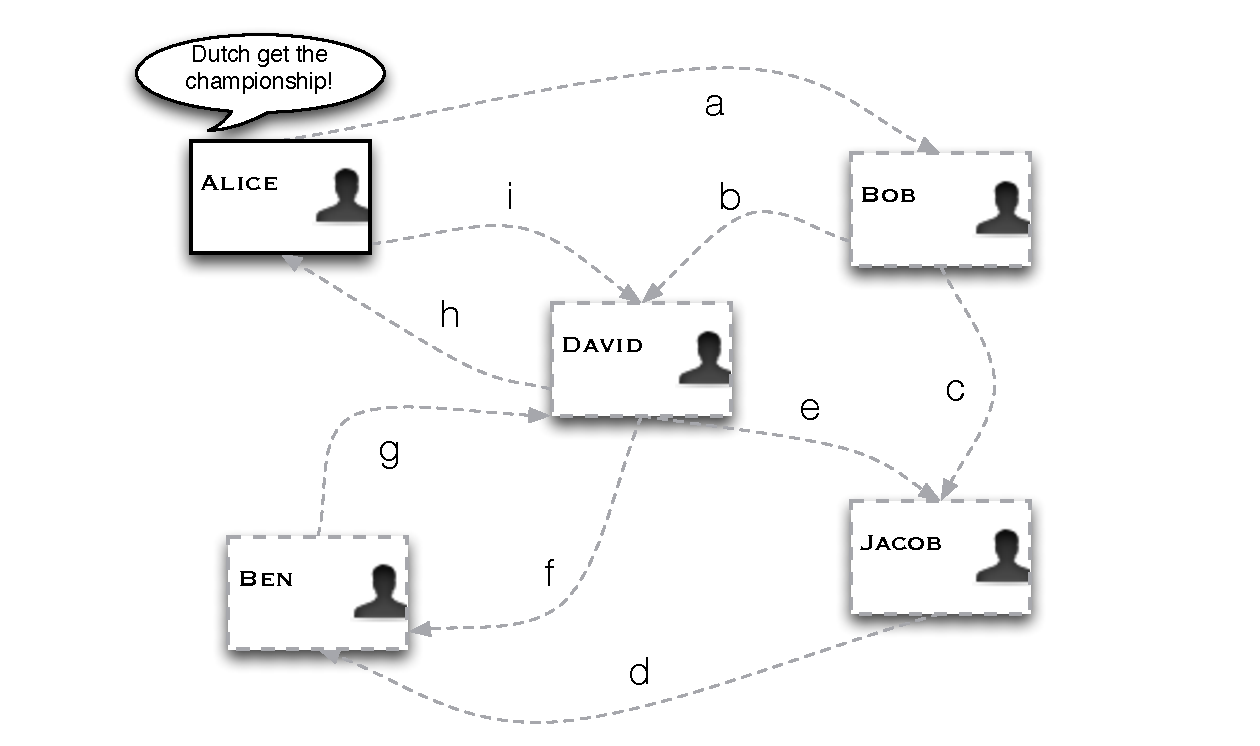
\includegraphics[scale=0.5]{./figures/motivation_2.pdf}}
	\only<3>{Bob sees the message and retweets the message from Alice. 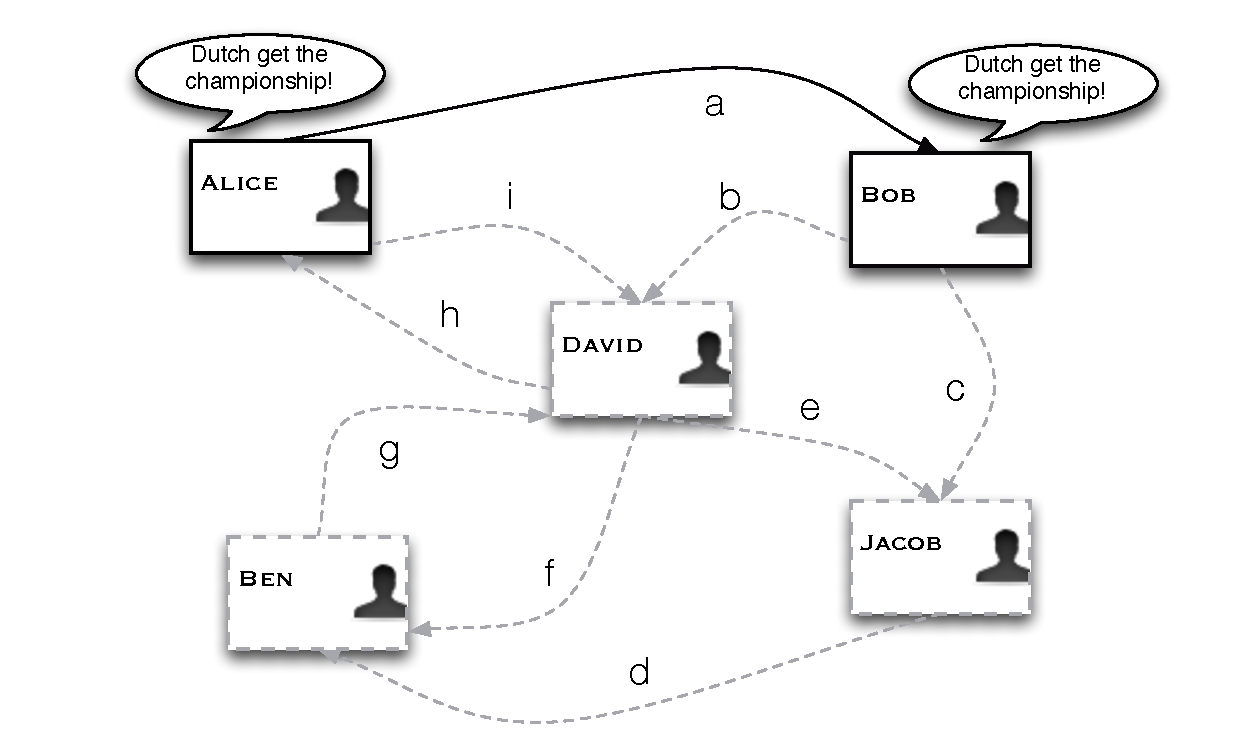
\includegraphics[scale=0.5]{./figures/motivation_3.pdf}}
	\only<4>{Jacob retweets the message from Bob. 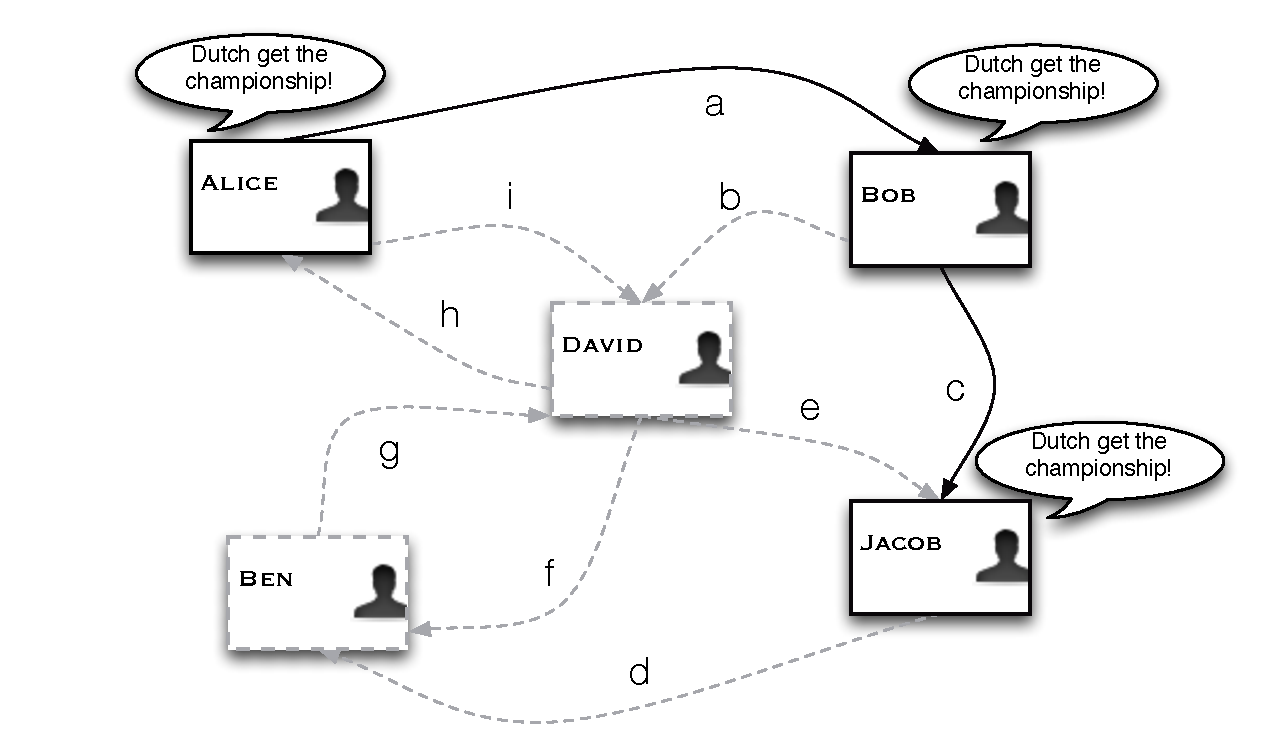
\includegraphics[scale=0.5]{./figures/motivation_4.pdf}}
	\only<5>{Ben retweets the message from Jacob. 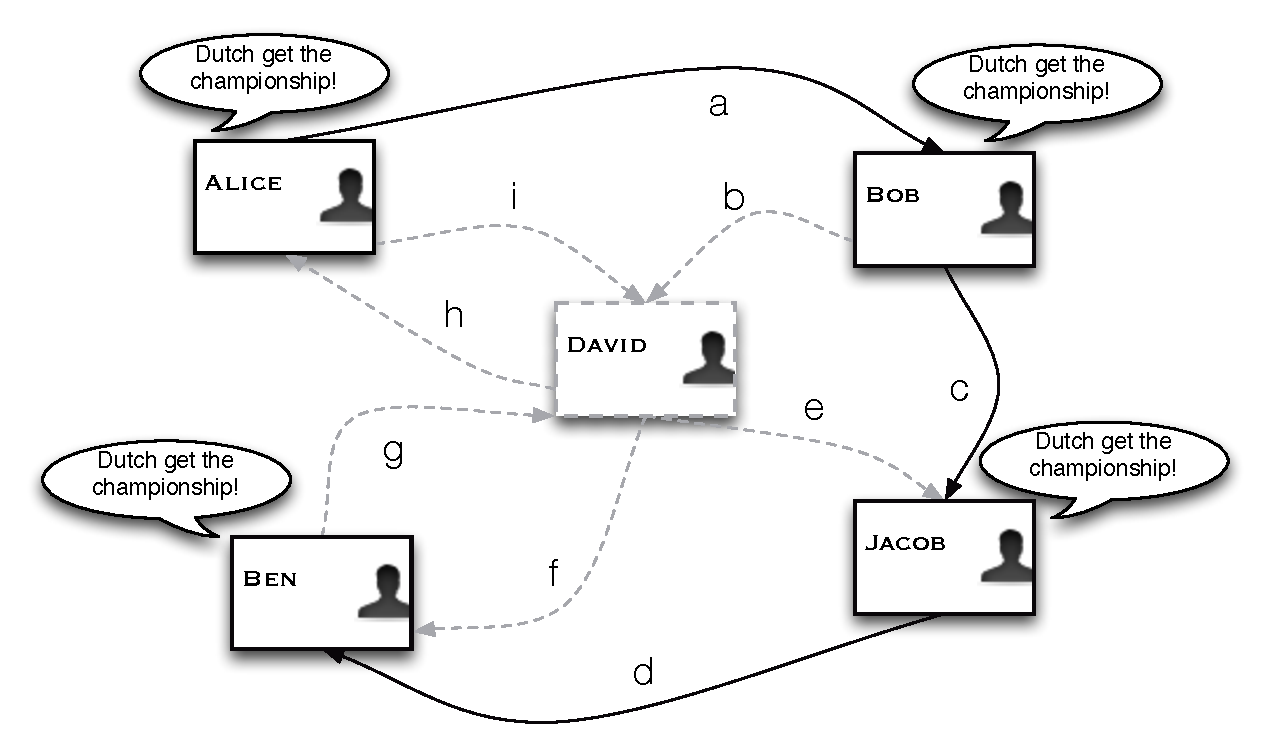
\includegraphics[scale=0.5]{./figures/motivation_5.pdf}}
	\only<6>{David is not a fan.  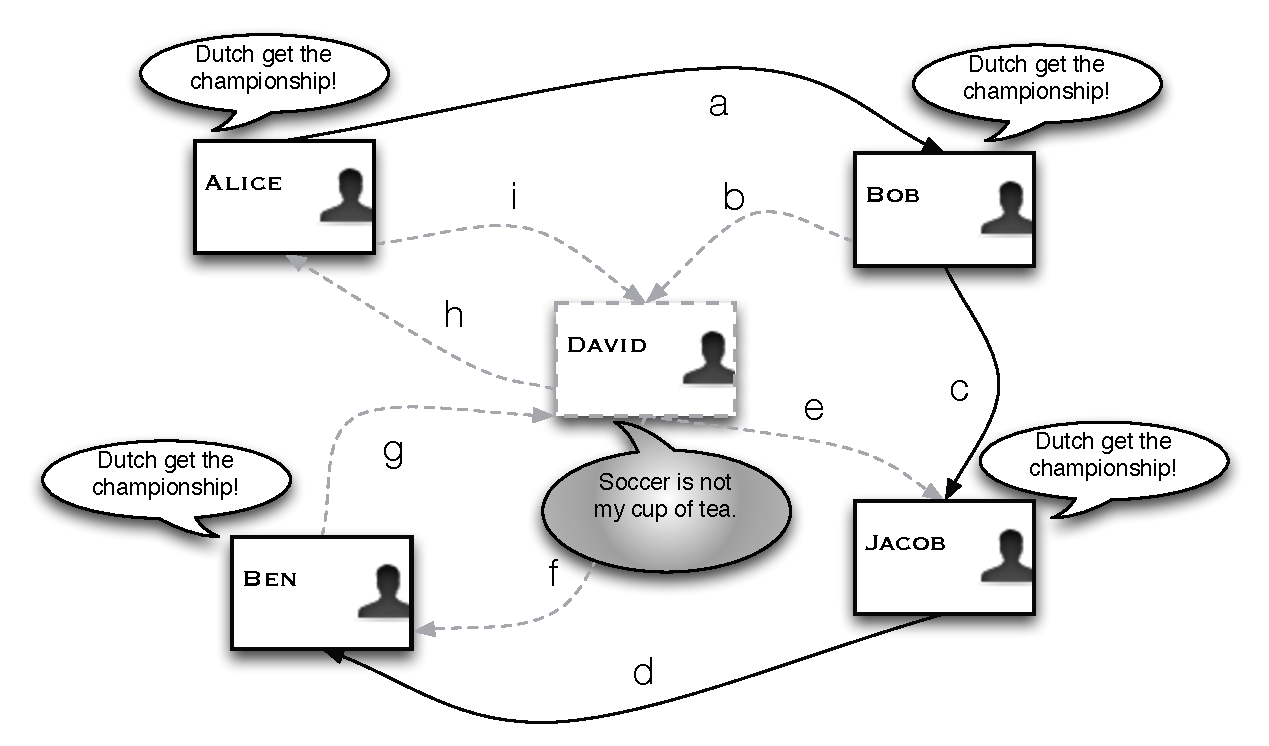
\includegraphics[scale=0.5]{./figures/motivation_6.pdf}}
\end{frame}


\begin{frame}{Network response problem}
	\begin{itemize}\footnotesize
		\item Definition:
		\begin{itemize}\footnotesize
			\item Given a complex network $G=(E,V)$, and an action $\vx$ performed on the network.
			\item Task: predict the subnetwork that responses to the action.
			\begin{itemize}\footnotesize
				\item Which nodes $v\in V$ perform the action? $V_{\vx}=\{Alice,Bob,Jacob,Ben\}$
				\item Which directed edges $e\in E_{\vx}$ relay the action from one node to its neighbors? $E_{\vx}=\{a,c,d\}$
			\end{itemize}
		\end{itemize}
	\end{itemize}
	\vspace{-10mm}
	\begin{figure}
		\center
		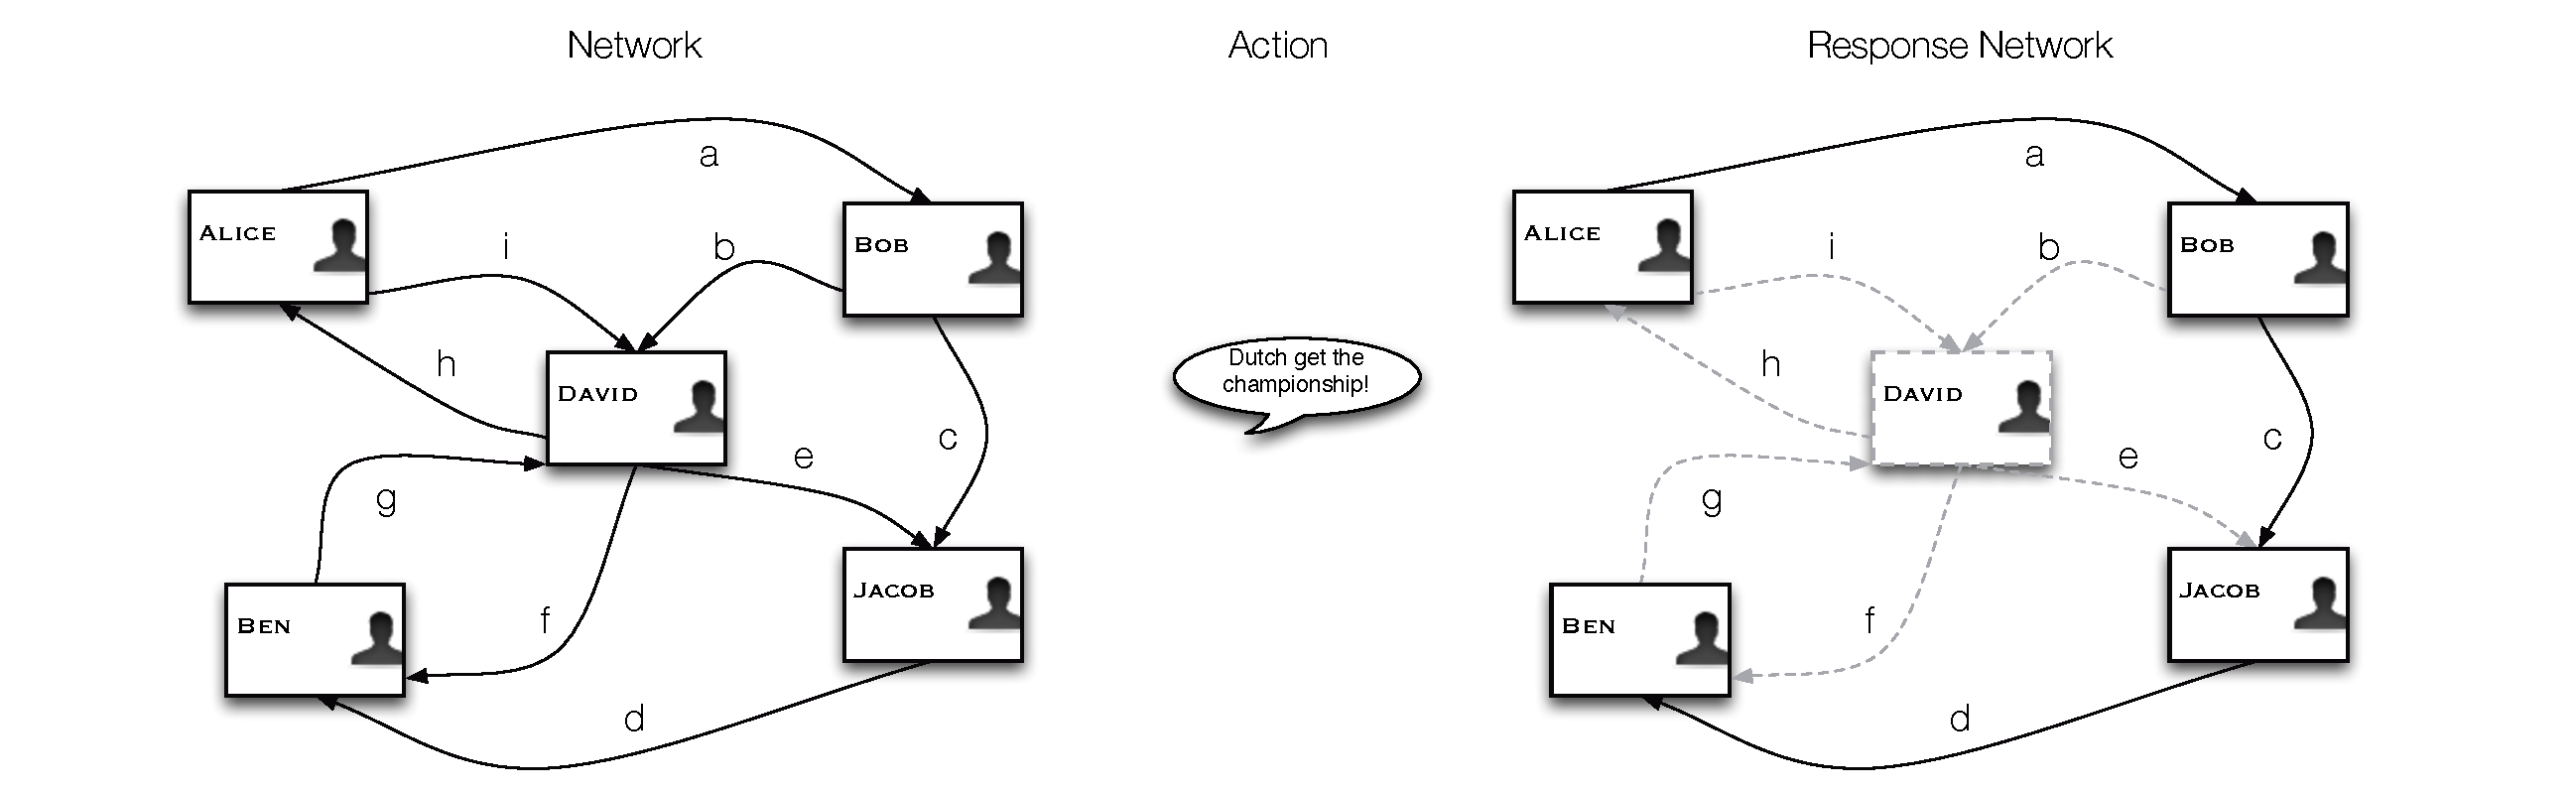
\includegraphics[scale=0.25]{./figures/problem_definition.pdf}
	\end{figure}
\end{frame}

\begin{frame}{Direct output graph}
	\begin{itemize}\footnotesize
		\item Model is defined on directed network.
		\begin{itemize}\footnotesize
			\item Any undirected network can be seen as special case by replacing undirected edges with two directed ones.
			\begin{figure}
				\center
				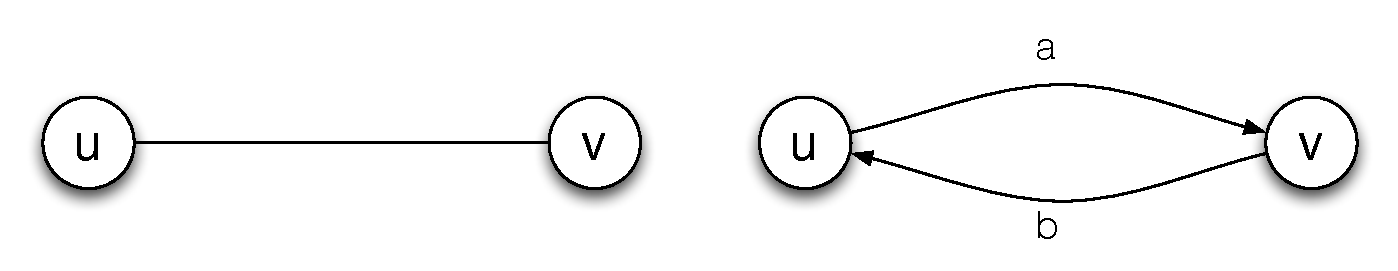
\includegraphics[scale=0.2]{./figures/model_definition.pdf}
			\end{figure}
		\end{itemize}
		\item Notation of edge labels:
		\begin{figure}
			\center
			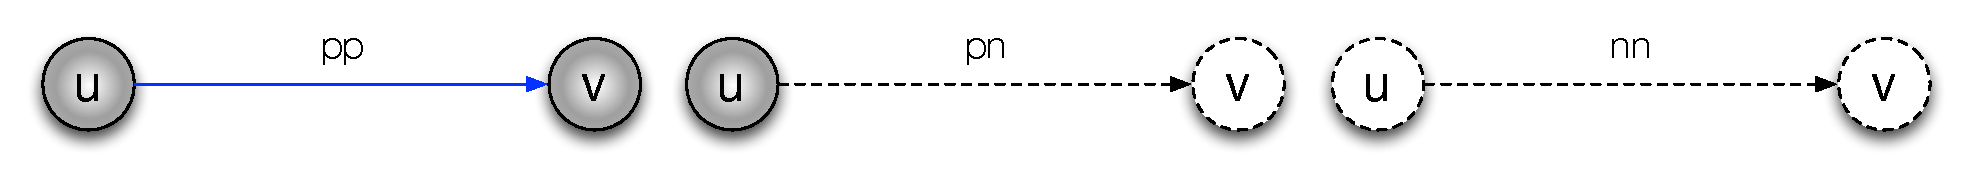
\includegraphics[scale=0.2]{./figures/notations.pdf}
		\end{figure}
		\item {\it Input feature}: Encode $\vx$ as $\varphib(\vx)$ (e.g. bag-of-word of a tweet).
		\item {\it Output feature}: Encode $G_{\vy}$ as $\psib(\vy)$ (e.g. a set of edges and their labels)
	\end{itemize}
	\begin{multicols}{2}
	{\scriptsize
		\begin{align*}
			&\psib(\vy) = \\
			& ( \underbrace{\underbrace{1}_{++}, \underbrace{0}_{+-}, \underbrace{0}_{--}}_{a}, 
			\underbrace{\underbrace{1}_{++}, \underbrace{0}_{+-}, \underbrace{0}_{--}}_{b},
			\underbrace{\underbrace{0}_{++}, \underbrace{1}_{+-}, \underbrace{0}_{--}}_{c},\cdots)
		\end{align*}}
	\begin{figure}
		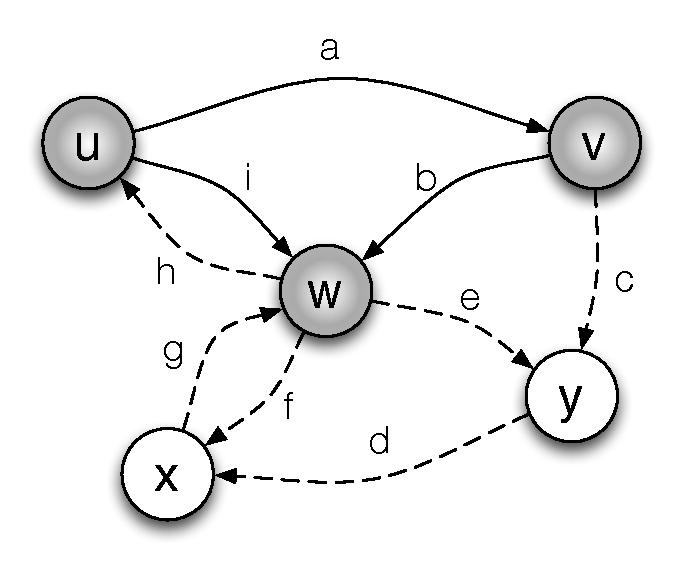
\includegraphics[scale=0.25]{./figures/propagation_example.pdf}
	\end{figure}
	\end{multicols}
\end{frame}

\begin{frame}{Structure output prediction model}
	\begin{itemize}
		\item Compatibility score for $(\vx,\vy)$: $F(\vx,\vy,\vw) = \ip{\vw}{\phib(\vx,\vy)}$
			\begin{itemize}\footnotesize
				\item $\vw$ is the feature weight to be learned.
				\item $\phib(\vx,\vy)=\varphib(\vx)\otimes\psib(\vy)$ is joint feature map.
				\item Intuition: given an action $\vx$, the score of correct response graph $(\vx,\vy)$ should be higher than any incorrect response graph $(\vx,\vy')$
				\begin{align*}
					F(\vx,\vy,\vw)>F(\vx,\vy',\vw), \quad \forall \vy'\in\Hcal(G).
				\end{align*}
			\end{itemize}
		\item $\vw$ is learned by solving structured output learning problem
		\begin{align*}
			\underset{\vw,\xi}{\minimize} &\quad \frac{1}{2}||\vw||^2_2+C\sum_{i=1}^{m}\xi_i \\
			\textbf{s.t.} &\quad F(\vx_i,\vy_i;\vw) > \underset{G_{\vx_i}'\in\Hcal(G)}{\maximize} (F(\vx_i,\vy_i', )\\
			&\quad +\ell_G(\vy_i,\vy_i'))-\xi_i, \xi_i\ge 0,\forall i\in\{1,\cdots,m\},
		\end{align*}
	\end{itemize}
\end{frame}

\begin{frame}{Inference problem}
	\begin{itemize}
		\item To solve the optimization, we have to solve similar inference problem appeared both in training and in prediction.
		\item In prediction phase:
		\begin{itemize}\footnotesize
			\item Given the feature weight $\vw$ and the complex network $G$.
			\item To find out a \daggraph\ $H^*=(V_H,E_H)$ that gives the maximal compatibility score for a given action $\vx$
		\end{itemize}
	\begin{align}
		H^*(\vx) = \underset{H\in \Hcal(G)}{\argmax}\, \sum_{e\in E^H}s_{\vy_e}(e,\vx,\vw).\label{spininference}
	\end{align}
	\begin{lemma}\footnotesize
		Finding the graph that maximizes Eq.~(\ref{spininference}) is an $\mathcal{NP}$-hard problem.
	\end{lemma}
	\begin{proof}\footnotesize
		Reduction from {\sc max-cut} problem.
	\end{proof}
	\end{itemize}
\end{frame}

\begin{frame}[allowframebreaks]{Approximate inference via {\sc SDP} relaxation}
	\begin{itemize}\footnotesize
		\item We formulate the inference problem as {\it integer quadratic program} ({\sc iqp}).
		\begin{itemize}\footnotesize
			\item Introduce for each node $u\in V$ a binary variable $x_u\in\{-1,+1\}$.
			\item Introduce a special variable $x_0\in\{-1,+1\}$ to distinguish activated node.
		\end{itemize}
		{\scriptsize
		\begin{align*}
		\maximize \; \frac{1}{4} \sum_{(u, v)\in E}\, [ & s_{\pn}(u,v) (1 + x_0 x_u - x_0 x_v - x_u x_v)  \\ 
			+ & s_{\nn}(u,v) (1 - x_0 x_u - x_0 x_v + x_u x_v)  \\ 
			+ & s_{\pp}(u,v) (1 + x_0 x_u + x_0 x_v + x_u x_v) ] \\
		\textbf{s.t.} \quad  x_0, x_u, x_v &\in \{-1,+1\}, \text{ for all } u,v\in V,
		\end{align*}}
		\item {\sc iqp} is relaxed into {\em quadratic program} ({\sc qp}) and solved by {\it semidefinite programming relaxation} ({\sc sdp}).
		\item Optimization guarantee $E[Z] \ge (\alpha-\epsilon) Z_{R} $ with $\alpha>0.796$, $Z$ is objective achieved by {\sc sdp}, $Z_R$ is objective of {\sc iqp}.
	\end{itemize}
\end{frame}

%
\begin{frame}{Short summary}
	\begin{itemize}\footnotesize
		\item We have seen so far. 
		\begin{tabular}{|c|c|c|}
			\hline
			\footnotesize
			 Output graph & Inference problem & Inference algorithm \\ \hline
			 Tree & Polynomial & DP \cite{Rousu07}  \\
			 Graph & \nphard & LBP \cite{su10structured}  \\ 
			 $\rightarrow$ \daggraph & \nphard & \sdp\ \cite{su14structured} \\ \hline
		\end{tabular}
		\item What if the output graph is not observed?
	\end{itemize}
\end{frame}
%
\begin{frame}{Research question}
	\begin{itemize}\footnotesize
		\item The output graph is hidden in many applications.
		\begin{itemize}\footnotesize
			\item For example, a surveillance photo can be tagged with ``building'', ``road'', ``pedestrian'', and ``vehicle''.
		\end{itemize}
		\item We study the problem in structured output learning when the output graph is not observed.
		\item In particular:
		\begin{itemize}\footnotesize
			\item Assume the dependency can be expressed by a complete set of pairwise correlations.
			\item Build a structured output learning model with a complete graph as the output graph.
			\item Solve the \nphard inference problem on the complete graph by a polynomial time algorithm.
		\end{itemize}
		\item A structured prediction model which performs max-margin learning on a random collection of spanning trees sampled from the output graph.
	\end{itemize}
\end{frame}

%
\begin{frame}{Complete graph as output graph}
	\begin{itemize}\footnotesize
		\item We assume that the joint feature map $\phib$ is a potential function on a Markov network (undirected graph) $G=(E,V)$.
		\item $G$ is a complete graph with $|V| = \ell$ nodes and $|E| = \frac{\ell(\ell-1)}{2}$ undirected edges.
		\item $G$ models all pairwise correlations.
		\item $\varphib(\vx)$ is the input feature map, e.g., bag-of-words feature of an example $\vx$.
		\item $\psib(\vy)$ is the output feature map which is a collection of edges and labels
		\begin{align*}\footnotesize
			\varphib(\vy) = (u_{e})_{e\in E},u_e\in\{-1,+1\}^2.
		\end{align*}
		\item The joint feature is the Kronecker product of $\varphib(\vx)$ and $\psib(\vy)$
		\begin{align*}\footnotesize
			\phib(\vx,\vy) = (\phib_e(\vx,\vy))_{e\in E}=(\varphib(\vx)\otimes\psib_e(\vy_e))_{e\in E}.
		\end{align*}
		\item The score function can be factorized by the complete graph $G$
		\begin{align*}
			F(\vw,\vx,\vy) = \ip{\vw}{\phib(\vx,\vy)} = \sum_{e\in E}\ip{\vw_e}{\phib_e(\vx,\vy_e)}.
		\end{align*}
	\end{itemize}
\end{frame}

\begin{frame}{Inference in terms of all spanning trees}
	\begin{itemize}
		\item Solving the following inference problem on a complete graph is \nphard
		\begin{align*}
			\vy_{\vw}(\vx) = \underset{\vy\in\vYcal}{\argmax}\,F(\vw,\vx,\vy)  = \underset{\vy\in\vYcal}{\argmax}\,\sum_{e\in E}\ip{\vw_e}{\phib_e(\vx,\vy_e)}. 
		\end{align*}
		$\phi_G(\vx,\vy) = \{\phi_{G,e}(\vx,\vy_e)\}_{e\in G},\vw_G = \{\vw_{G,e}\}_{e\in G},||\phi_G(\vx,\vy)||=||\vw_{G}||=1$
		\item For a complete graph, there are $\ell^{\ell-2}$ unique spanning trees.
		\item $\phi_T(\vx,\vy)=\{\phi_e(\vx,\vy)\}_{e\in T}$ is the projection of $\phi_G(\vx,\vy)$ on $T\in S(G)$.
		\item $\vw_{T}=\{\vw_{G,e}\}_{e\in T}$ is the projection of $\vw_G$ on $T\in S(G)$.
		\item We can write $F(\vw,\vx,\vy)$ as a conic combination of all spanning trees
		\begin{align*}
			F(\vw,\vx,\vy) &= \underset{T\in U(G)}{\E}a_T\ip{\vw_T}{\phib_T(\vx,\vy)}\\
			  &\underset{T\in U(G)}{\E}a_T^2=1,  \underset{T\in U(G)}{\E}a_T<1.
		\end{align*}
		\item $U(G)$ is the uniform distribution over $\ell^{\ell-2}$ spanning trees.
		\item The number of spanning trees is exponentially dependent on the number of nodes $\ell$.
	\end{itemize}
\end{frame}

%
\begin{frame}{A sample of $n$ spanning trees}
	\begin{itemize}\footnotesize
		\item Instead of using all spanning trees, we can just use $n$ spanning trees
		\begin{align*}\footnotesize
			F_{\Tcal}(\vw,\vx,\vy) &= \frac{1}{n}\sum_{i=1}^{n}a_{T_i}\ip{\vw_{T_i}}{\phib_{T_i}(\vx,\vy)}\\
			  &\frac{1}{n}\sum_{i=1}^{n}a_{T_i}^2=1,  \frac{1}{n}\sum_{i=1}^{n}a_{T_i}<1.
		\end{align*}
		\item When
		\begin{align*}\footnotesize
			n\ge\frac{\ell^2}{\epsilon^2}(\frac{1}{16}+\frac{1}{2}\ln\frac{8\sqrt{n}}{\delta}),
		\end{align*}
		we have $|F_{\Tcal}(\vw,\vx,\vy)-F(\vw,\vx,\vy)|\le\epsilon$, with high probability.
		\item A sample of $n\in\Theta(\ell^2/\delta^2)$ random spanning tree is sufficient to estimate the score function.
		\item Margin achieved by $F(\vw,\vx,\vy)$ is also preserved by the sample of $n$ random spanning trees $F_{\Tcal}(\vw,\vx,\vy)$ \cite{su14multilabelnips}.
	\end{itemize}
\end{frame}

%
\begin{frame}{Random spanning tree approximation \rta}
	\begin{itemize}\footnotesize
		\item The optimization problem of \rta\ is defined as \cite{su14multilabelnips}
		\begin{align*}
			\underset{\vw_{T_i},\xi_i}{\minimize} & \quad \frac{1}{2}\sum_{i=1}^{n}\norm{\vw_{T_i}}^2 + C\sum_{k=1}^{m}\xi_k\\
			\st & \quad \frac{1}{\sqrt{n}}\sum_{i=1}^{n}{ \langle \vw_{T_i}, \phib_{T_t}(\vx_k,\vy_k) \rangle} - \underset{\vy \neq \vy_k}{\maximize\ } \frac{1}{\sqrt{n}}\sum_{i=1}^{n}{\langle \vw_{T_t}, \phib_{T_i}(\vx_k,\vy) \rangle } \geq 1 -  \xi_k, \\
			& \quad \xi_k\ge0\, , \forall\ k \in \set{1,\dots,m}.
		\end{align*}
		\item The marginal-dual form is given by
		\begin{align*}\footnotesize
			\underset{\vmu\in\Mcal}{\maximize} & \quad \sum_{i=1}^{n}\left( \vmu_{T_i}\vell_{T_i} - \frac{1}{2}\vmu_{T_i}K^{\Delta\phib}_{T_i}\vmu_{T_i}\right)\\
			\st & \quad \sum_{u_e}\vmu_{T_i,e}(u_e)\le C.
		\end{align*}
		\item Inside the summation, there is a structure output model with parameter $\vmu_{T_i}$ defined on a spanning tree $T_i$.
		\item The problem is how to jointly optimize structured output models defined on $n$ spanning trees.
	\end{itemize}
\end{frame}

%
\begin{frame}{Inference problem for a collection of trees}
	\begin{itemize}
		\item The inference problem of \rta\ is defined as finding the multilabel $\vy_{\Tcal}(\vx)$ that maximizes the sum of scores over a collection of trees
		\begin{align*}
			\vy_{\Tcal}(\vx) = \underset{\vy\in\vYcal}{\argmax}\,{\color{aaltoblue}F_{\Tcal}(\vx,\vy;\vw_{\Tcal})} = \underset{\vy\in\vYcal}{\argmax}\,\sum_{t=1}^{n}\ip{\vw_{T_t}}{\phi_{T_t}(\vx,\vy)}.
		\end{align*}
		\item The inference problem on each individual spanning tree can be solve efficiently in $\Theta(\ell)$ by \textit{dynamic programming}
		\begin{align*}
			\vy_{T_t}(\vx) = \underset{\vy\in\vYcal}{\argmax}\,{\color{aaltored}F_{T_t}(\vx,\vy;\vw_{T_t})}= \underset{\vy\in\vYcal}{\argmax}\,\ip{\vw_{T_t}}{\phi_{T_t}(\vx,\vy)}.
		\end{align*}
		\item There is no guarantee that there exists a tree $T_t\in\Tcal$ in which the maximizer of ${\color{aaltored}F_{T_t}}$ is the maximizer of ${\color{aaltoblue}F_{\Tcal}}$.
	\end{itemize}
\end{frame}

%
\begin{frame}[allowframebreaks]{Fast inference for a collection of trees}
	\begin{itemize}
		\item For each tree $T_t$, instead of computing the best multilabel $\vy_{T_t}$, we compute $K$-best multilabels in $\Theta(K\ell)$ time
		\begin{align*}
			\Ycal_{T_t,K} = \{\vy_{T_t,1},\cdots,\vy_{T_t,K}\}.
		\end{align*}
		\item Performing the same computation on all trees gives a candidate list of $n\times K$ multilabels (K best list) in $\Theta(nK\ell)$ time
		\begin{align*}
			\Ycal_{\Tcal,K}=\Ycal_{T_1,K}\cup\cdots\Ycal_{T_n,K}.
		\end{align*}
		\item We prove that with high probability the global best multilabel will exist in K best list.
		\item We have developed a condition to verify the global best multilabel from K best list in linear time $\Theta(nK)$.
	\end{itemize}
\end{frame}

\iffalse
\begin{frame}{Exact line search for a single tree}
	\begin{figure}
		\begin{center}
			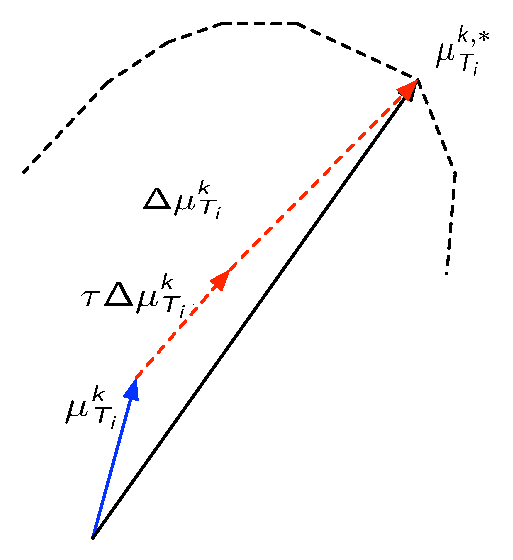
\includegraphics[scale=0.3]{optimization_single_tree.pdf}
		\end{center}
	\end{figure}
	\begin{itemize}
		\item Line search gives the optimal feasible solution as a stationary point ($\tau$)
		\begin{align}
			\underset{\tau}{\maximize} &\quad f(\vmu_{T_i}^k + \tau\Delta\vmu_{T_i}^{k})\label{tree_line_search}\\
			\st &\quad 0\le\tau\le1.\nonumber
		\end{align}
		\item $\tau=0$ corresponds to no update.
		\item Feasible maximum update is achieved at $\tau=1$. 
	\end{itemize}
\end{frame}

\begin{frame}{Optimization on a collection of $n$ spanning trees}
	\begin{figure}
		\begin{center}
			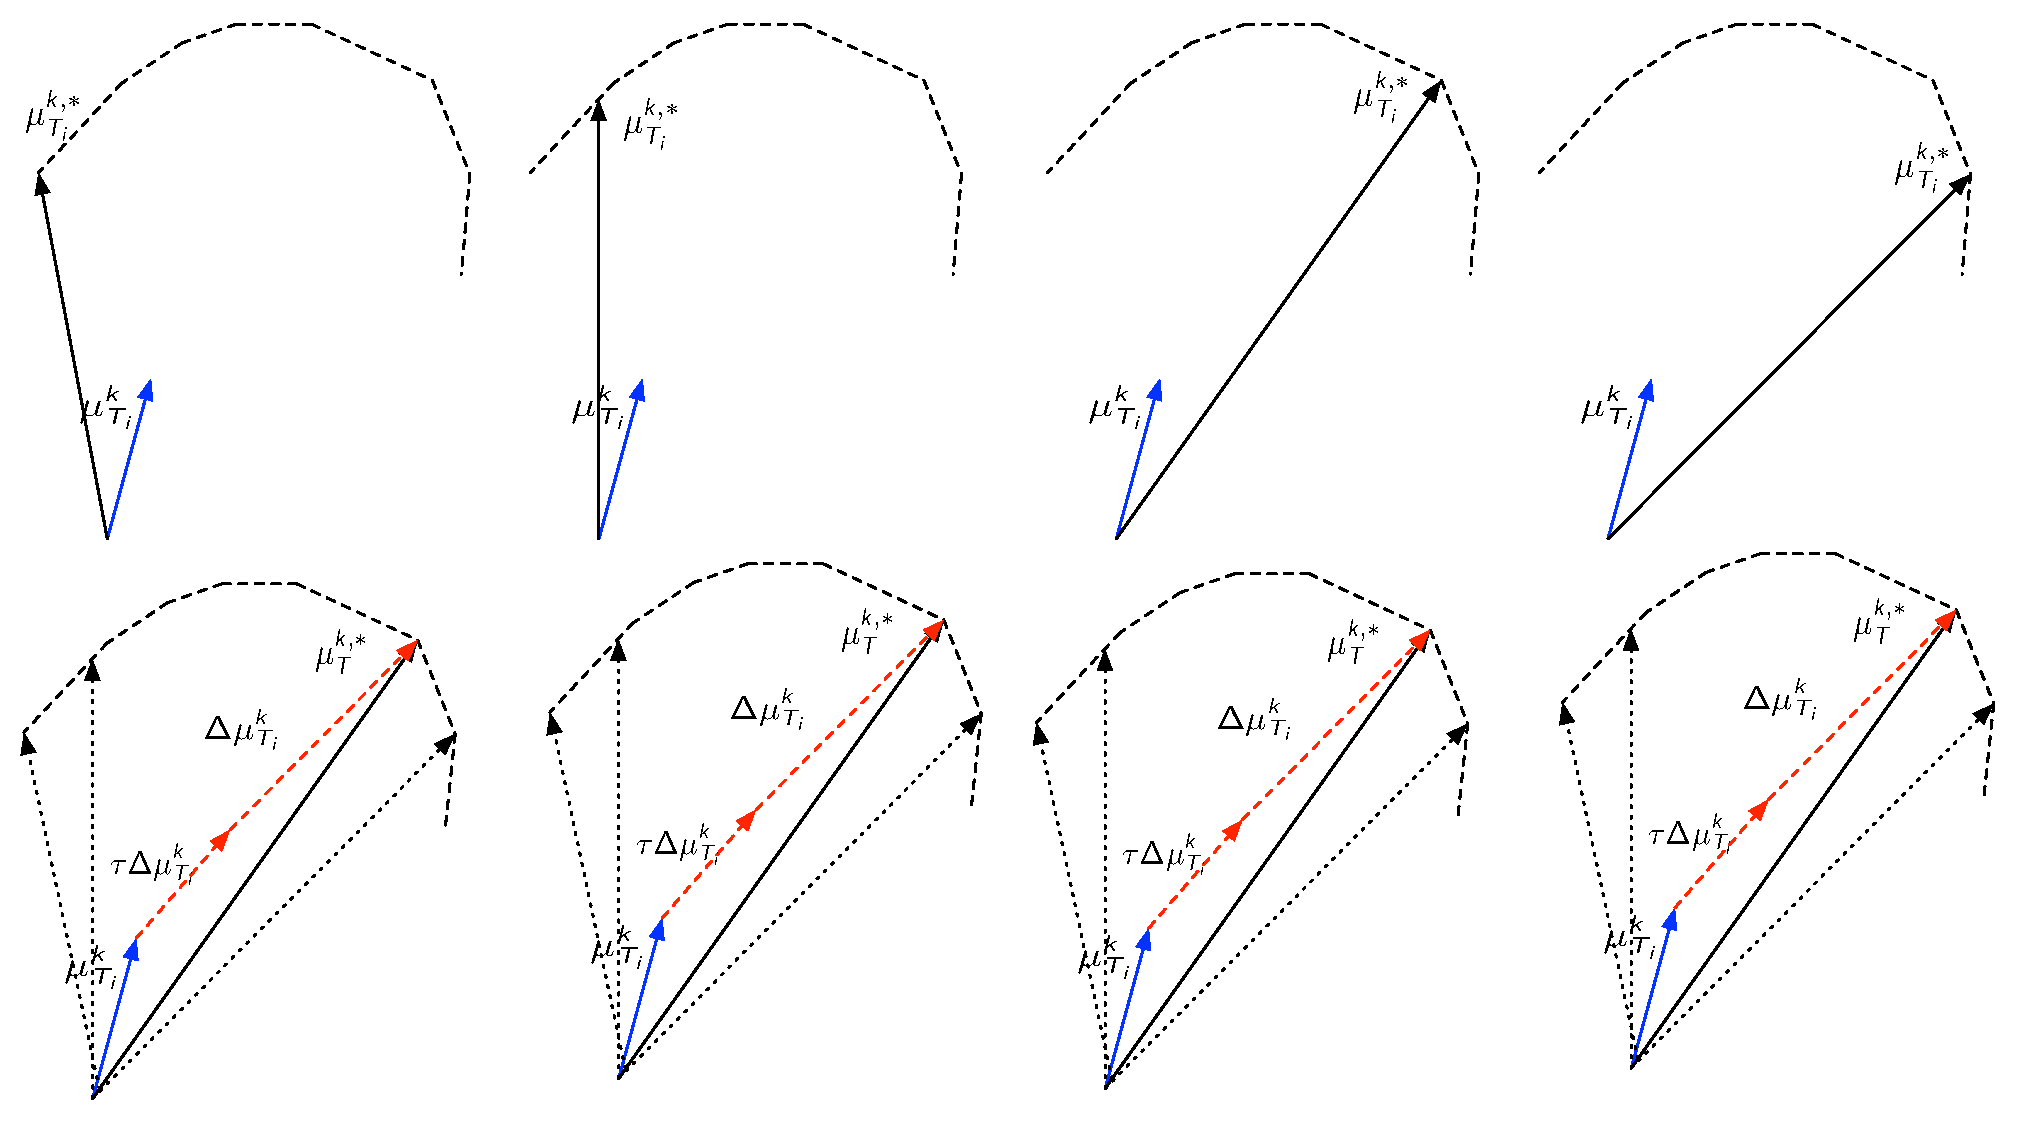
\includegraphics[scale=0.3]{best_update.pdf}
		\end{center}
	\end{figure}
\end{frame}

\begin{frame}{Exact line search for the collection of trees}
	\begin{itemize}
		\item The step size along the update direction $\tau$ is given by the exact line search
		\begin{align*}\footnotesize
			\underset{\tau}{\maximize} &\quad {\color{aaltored}\sum_{i=1}^n}f(\vmu_{T_i}^k + \tau\Delta\vmu_{T_i}^{k})\\
			\st &\quad 0\le\tau\le1.
		\end{align*}
		\item Problems with the {\em best update}
		\begin{enumerate}\footnotesize
			\item The best feasible solution on a single tree might not be the best feasible solution on a collection of trees
			\begin{align*}
				{\vmu}_{T}^{k,*}\notin{\color{aaltored}{}{\vmu}_{T_i}^{k,*}{\color{aaltored}}_{i=1}^n}.
			\end{align*}
			\item $\kappa$-best inference algorithm
			\begin{align*}
				({\vmu}_{T_i}^{k,*_h})_{h=1}^{\kappa} &= \underset{\vmu\in\Mcal}{\argmax}\,\vmu\tp g_{T_i}^k,\,{\color{aaltored}\forall i}\\
				{\vmu}_{T}^{k,*} &\in {\color{aaltored}{}{\vmu}_{T_i}^{k,*_h}{\color{aaltored}}_{i=\{1,\cdots,n\},h\in\{1,\cdots,\kappa\}}}.
			\end{align*}
		\end{enumerate}
	\end{itemize}
\end{frame}

\begin{frame}{Update with multiple directions}
	\begin{figure}
		\begin{center}
			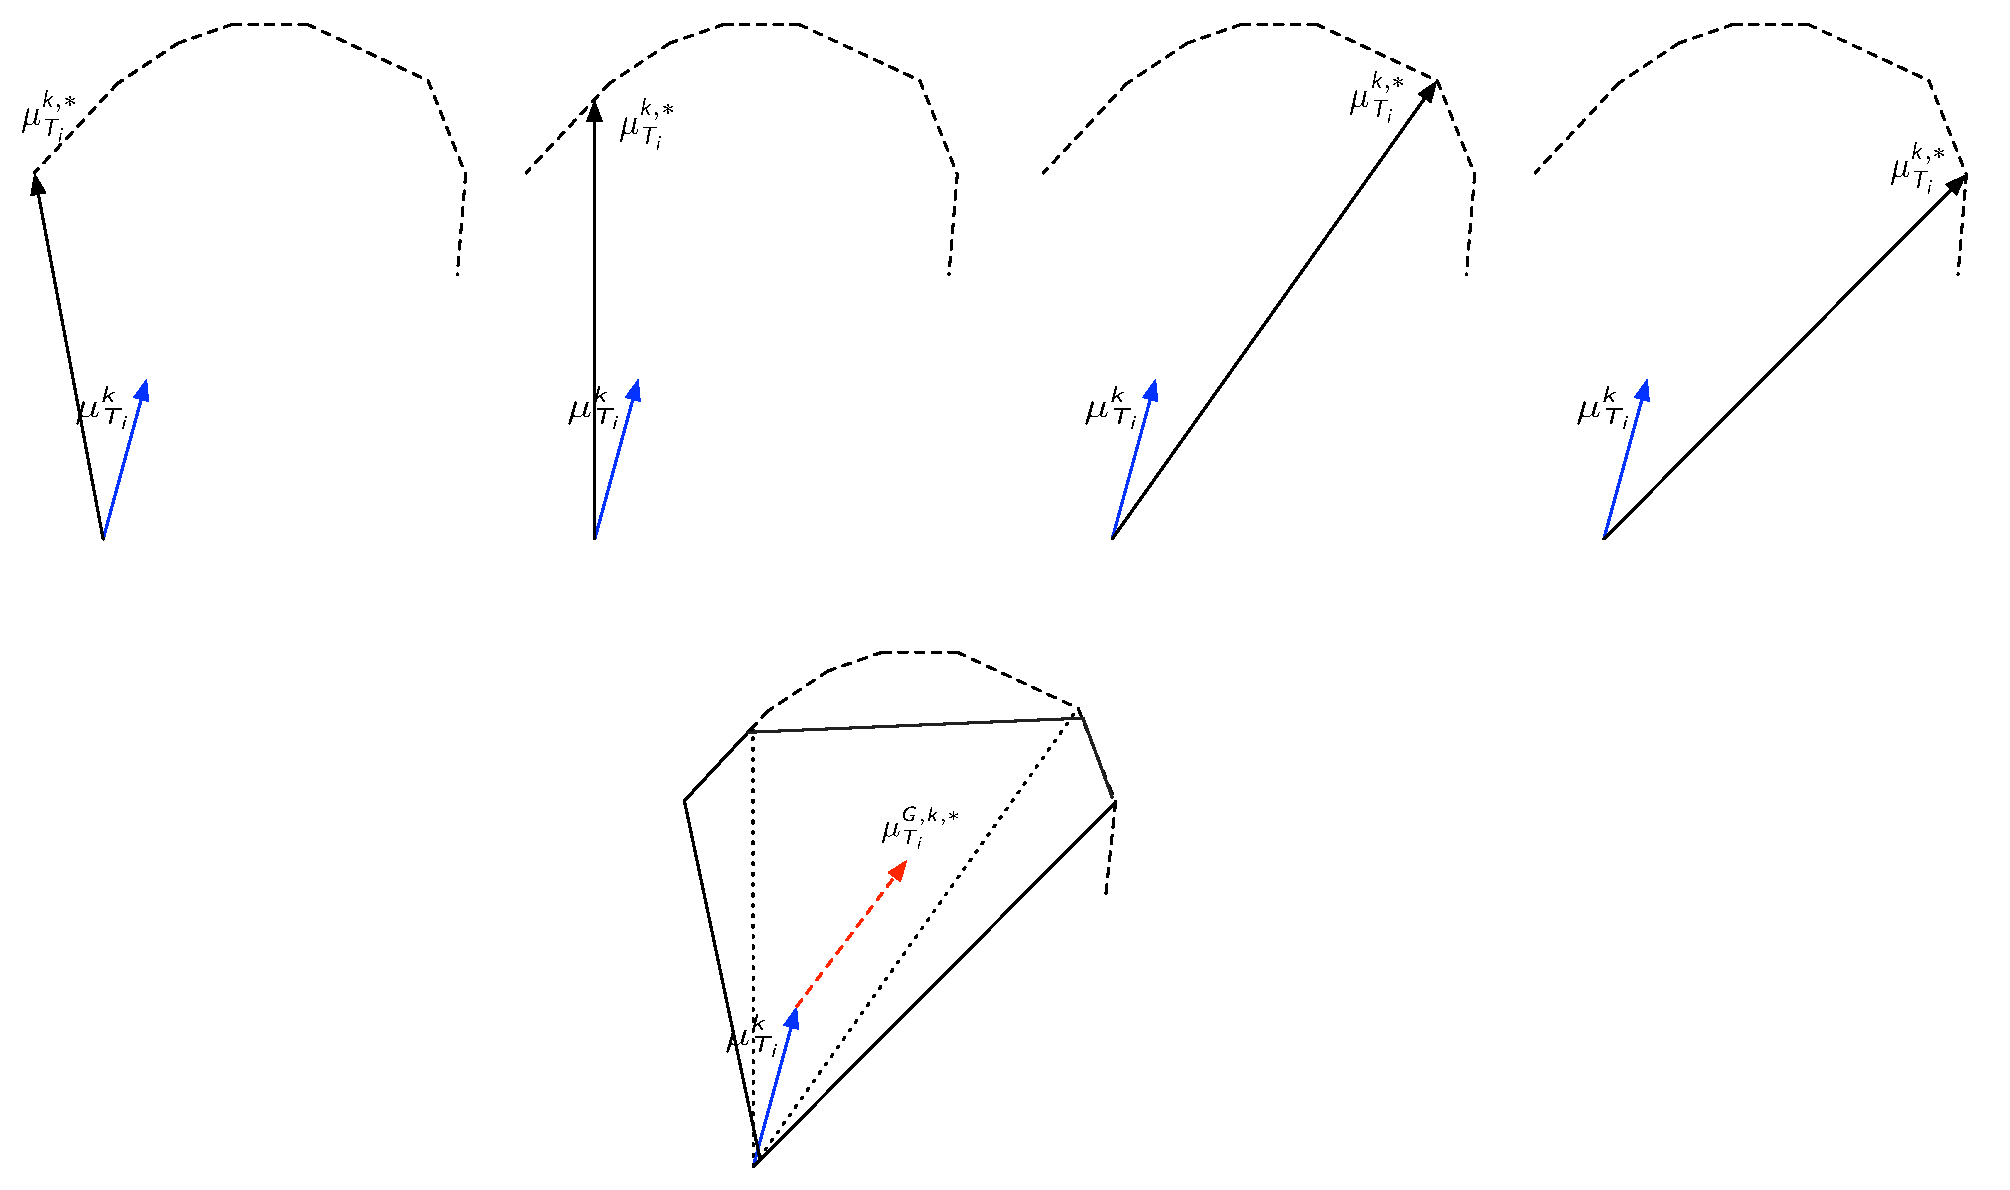
\includegraphics[scale=0.3]{multiple_update.pdf}
		\end{center}
	\end{figure}
\end{frame}

\begin{frame}{Newton method to compute $\vtau$}
	\begin{itemize}\footnotesize
		\item We want to find $\tau$ that maximize the objective function given the update
		% \begin{align*}\footnotesize
		% 	&f(\vmu^{G,k} + \Delta{\vmu}^{G,k+1}) \\
		% 	&= (\vmu^{G,k} + \Delta{\vmu}^{G,k+1})\tp\ell_G - \frac{1}{2}(\vmu^{G,k} + \Delta{\vmu}^{G,k+1})\tp K_G (\vmu^{G,k} + \Delta{\vmu}^{G,k+1}).
		% \end{align*}
		\begin{align*}
			\underset{\tau}{\maximize} & \quad f(\vmu^{G,k} + \Delta{\vmu}^{G,k+1})\\
			\st & \quad 0\le\tau_i\le1,\,\sum_{i=1}^n\tau_i\le1,\,\forall i.
		\end{align*}
		\item The objective is quadratic with respect to $\vtau$.
		\item We use Newton method to find $\vtau$ that maximize the objective.
		\item $\vtau$ is projected into the feasible region.
	\end{itemize}
\end{frame}
\fi

\begin{frame}{Short summary}
	\begin{itemize}\footnotesize
		\item We have seem so far.		
	\end{itemize}
		\begin{tabular}{|c|c|p{5.5cm}|}
			\hline
			\footnotesize
			 Output graph & Inference problem & Inference algorithm \\ \hline
			 Tree & Polynomial & DP \cite{Rousu07}  \\
			 Graph & \nphard & LBP \cite{su10structured}  \\ 
			 \daggraph & \nphard & \sdp\ \cite{su14structured} \\ 
			 $\rightarrow${unknown} & \nphard & \mve\ \amm\ \mam\ \cite{su15multilabel} \rta\ \cite{su14multilabelnips} \\ \hline
		\end{tabular}
\end{frame}

%
\begin{frame}{\rta\ inference algorithm}
	\begin{itemize}\footnotesize
		\item $10$ datasets, $|\Tcal| = \{5,10,40\}, K=\{2,4,8,16,32,40,60\}$.
		\item Y-axis is the percentage of examples with exact inference.
		\item X-axis is the value of $K$ as the percentage of the number of microlabels.
		\item $K=100\%|Y|$ corresponds to a complexity of $\Theta(n\ell^2)$.
	\end{itemize}
	\begin{figure}
		\begin{center}
			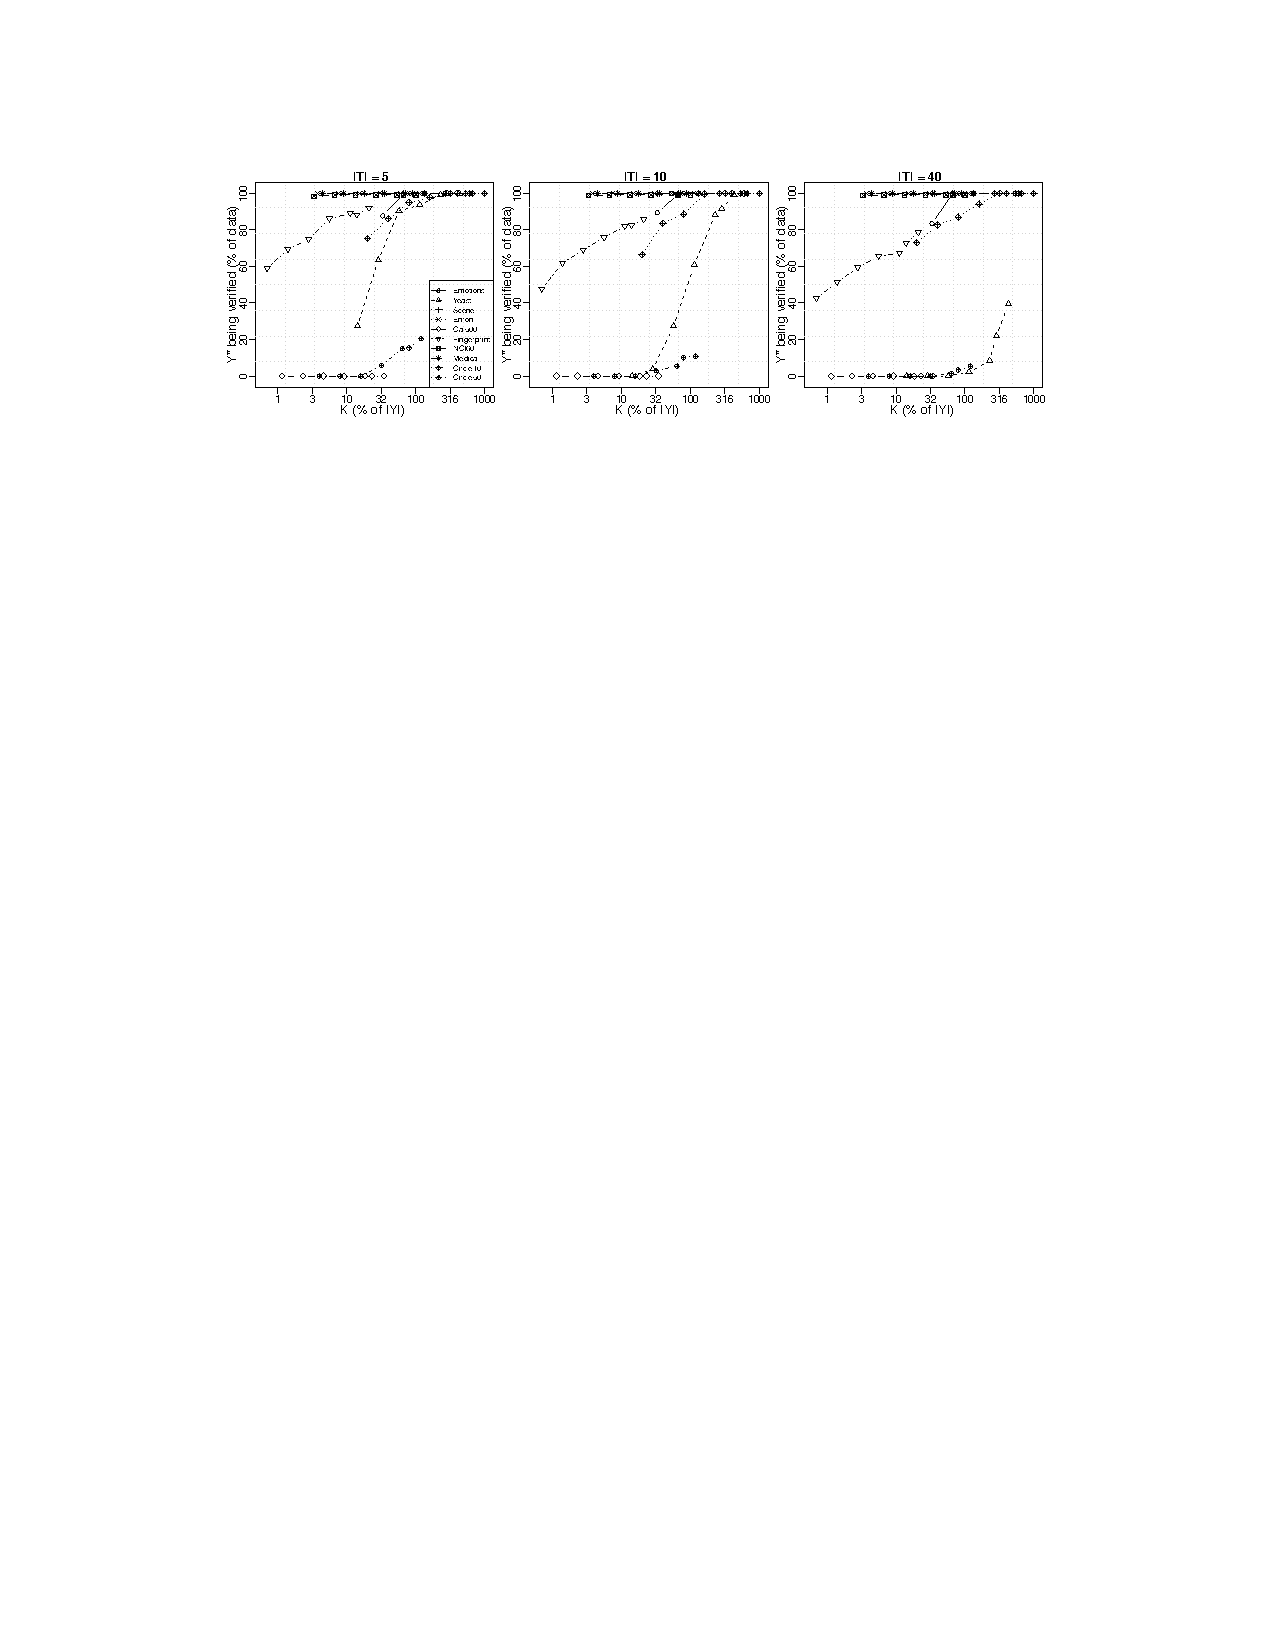
\includegraphics[width=11cm]{./result_plot.pdf}
			%\caption{Percentage of examples with provably optimal $\vy$ being in the $K$-best lists plotted as a function of K, scaled with respect to the number of microlabels in the dataset.}
		\end{center}
	\end{figure}
\end{frame}



%
\begin{frame}{\rta\ on multilabel benchmark datasets}
	\begin{itemize}\footnotesize
		\item Prediction performance on multilabel benchmark datasets.
		\item Measurement of success is microlabel accuracy and multilabel accuracy.
		\item The result is shown in the following table.
	\end{itemize}
	\begin{figure}\footnotesize
		\begin{center}
			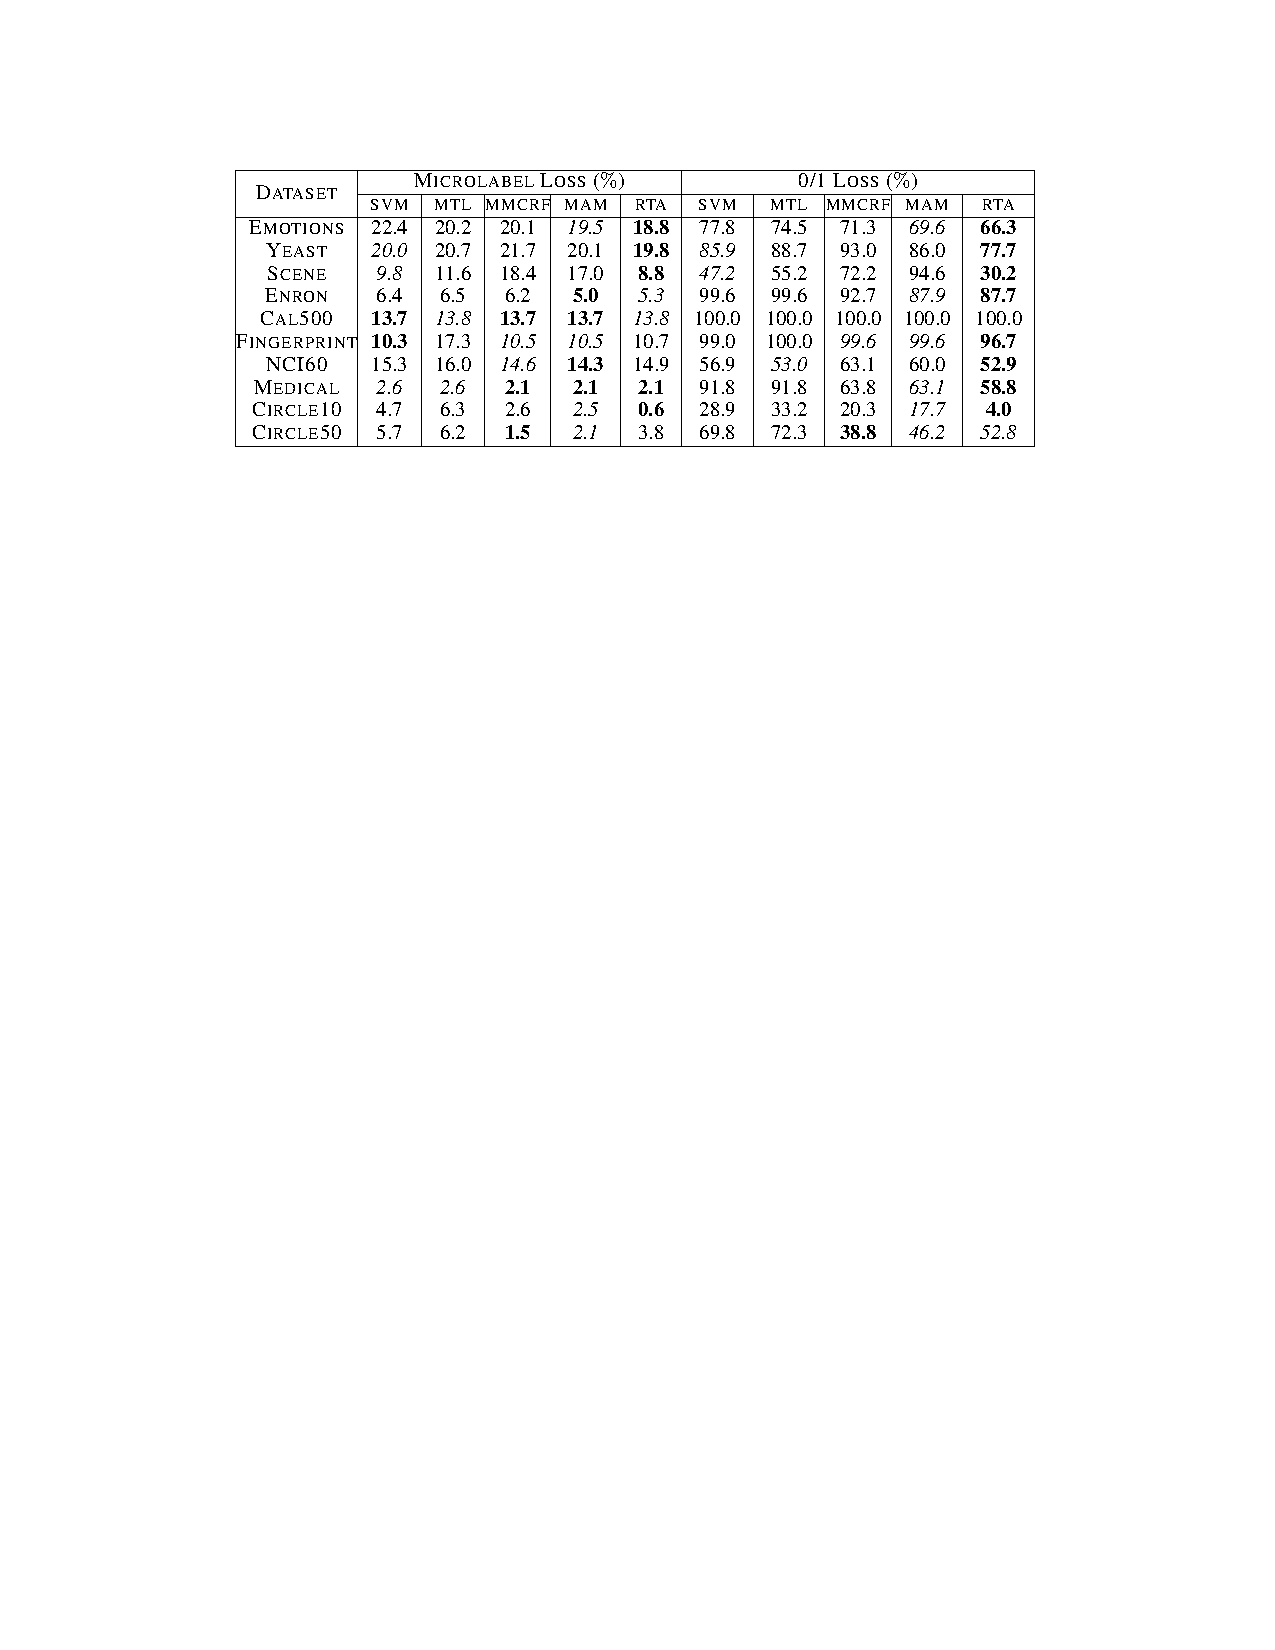
\includegraphics[width=11cm]{./result_table.pdf}
		\end{center}
	\end{figure}
\end{frame}


\begin{frame}{\spin\ for context-sensitive prediction}
	\begin{itemize}\footnotesize
		\item We assume action $\varphib(\vx)$ is known (e.g. bag-of-word of a tweet).
		\item Task is to predict the response network given the action.
		%\item {\em Predicted Subgraph Coverage} (PSC) is defined as $\mathrm{PSC}=\frac{1}{mn} \sum_{i=1}^{m} \sum_{v\in V_i} |G_v|$.
		\item {\em Predicted Subgraph Coverage} (PSC) is the relative size of correctly predicted subgraph in terms of node labels.
		\item The result is shown in the following table.
	\end{itemize}	
		\begin{table}[t]
		\scriptsize
		\centering
		\begin{tabular}{|@{  }c@{  }|@{}c@{  }c@{  }c@{}|@{}c@{  }c@{  }c@{}|@{}c@{ }c@{}|@{}c@{  }c@{  }c@{}|}
		  \hline
		\multirow{2}{*}{\textbf{Dataset}} & \multicolumn{3}{c}{\textbf{Node Accuracy}} & \multicolumn{3}{|c}{\textbf{Node $F_1$ Score}} & \multicolumn{2}{|c}{\textbf{Edge Acc}} & \multicolumn{3}{|c|}{{\em PSC}}  \\ \cline{2-12}
		 & \scriptsize{SVM} & \scriptsize{MMCRF} & \scriptsize{SPIN} & \scriptsize{SVM} & \scriptsize{MMCRF} & \scriptsize{SPIN} & \scriptsize{SVM}  & \scriptsize{SPIN}  & \scriptsize{SVM} & \scriptsize{MMCRF} & \scriptsize{SPIN}  \\ \hline
		   memeS  & \textbf{73.4} & {68.0} & \em{72.2} & {39.0} & \em{39.8} & \textbf{47.1} & \textbf{62.7} & {45.6} & {23.4} & \em{25.3} & \textbf{33.6} \\ 
		   memeM  & \textbf{82.1} & {79.0} & \em{81.5} & {29.1} & \em{30.1} & \textbf{38.0} & {61.1} & \textbf{68.8} & {18.6} & \em{18.8} & \textbf{28.3} \\ 
		   memeL  & \textbf{89.9} & {88.3} & \em{89.8} & {26.7} & \em{27.1} & \textbf{35.0} & {45.5} & \textbf{80.0} & {17.7} & \em{18.9} & \textbf{27.6} \\ 
		%M100  & {71.2} & \em{73.6} & \textbf{76.7} & {49.3} & \em{50.8} & \textbf{54.3} & {33.3} & \textbf{61.7} & {33.3} & \textbf{35.6} & \em{34.6} & \textbf{0.1} & {0.2} & \textbf{0.1}\\ 
		%M500  & {89.0} & \em{91.4} & \textbf{92.0} & \textbf{18.8} & {13.5} & \em{14.6} & {28.2} & \textbf{92.6} & \em{29.3} & {26.4} & \textbf{29.5} & {9.0} & \em{3.8} & \textbf{3.2}\\ 
		M700  & {91.9} & \textbf{94.1} & \em{92.1} & \em{13.8} & {7.3} & \textbf{14.2}  & {26.3} & \textbf{93.0} & \em{29.4} & {23.9} & \textbf{34.4} \\ 
		M1k & {94.1} & \textbf{95.8} & \em{94.2} & \textbf{10.9} & {3.5} & \em{9.3}   & {26.6} & \textbf{94.7} & \em{33.7} & {16.6} & \textbf{35.2} \\ 
		M2k & \em{96.8} & \textbf{97.6} & {96.7} & \textbf{6.2} & {1.4} & \em{3.4}    & {25.3} & \textbf{97.6} & \textbf{34.6} & {9.6} & \em{14.7} \\ 
		%L100  & {69.4} & \em{72.2} & \textbf{75.7} & {51.1} & \em{53.1} & \textbf{57.4} & {31.6} & \textbf{62.3} & {30.9} & \em{31.7} & \textbf{33.4} & \textbf{0.1} & \em{0.2} & {0.3}\\ 
		%L500  & {85.9} & \textbf{89.1} & \em{86.8} & \em{21.7} & {15.1} & \textbf{24.7} & {27.9} & \textbf{87.9} & \em{14.2} & {11.2} & \textbf{19.7} & {6.5} & \em{3.2} & \textbf{2.1}\\ 
		L700  & {89.7} & \textbf{92.4} & \em{89.7} & \em{16.2} & {9.4} & \textbf{17.3}  & {26.5} & \textbf{90.4} & \em{9.5} & {6.7} & \textbf{12.5} \\ 
		L1k & \em{92.4} & \textbf{94.4} & {91.5} & \em{12.4} & {6.4} & \textbf{13.9}  & {26.4} & \textbf{92.3} & \em{6.1} & {4.4} & \textbf{8.4} \\ 
		L2k & \em{92.5} & \textbf{94.5} & {91.9} & \em{12.3} & {5.4} & \textbf{12.7}  & {26.5} & \textbf{93.2} & \em{6.0} & {2.9} & \textbf{7.2} \\ \hline
		\textbf{Geom.}  & {85.5} & \em{86.4} & \textbf{86.6} & \em{19.8} & {12.6} & \textbf{20.3} & {32.6} & \textbf{79.7} & \em{18.9} & {14.2} & \textbf{21.7} \\
		\hline
		\end{tabular}
		\label{table_global_res_svm}
		\end{table}
\end{frame}

\begin{frame}{\spin\ for context-free prediction}
	\begin{itemize}
		\item We assume action is unknown during prediction phase.
		\item Task is to predict directed edges (network skeleton) from a cascade of actions.
		\item The measure of success is {\em Precision@$K$}, where we ask for top-$K$ percent edge predictions and compute the precision.
		\item The result is shown in the following table.
	\end{itemize}
			\begin{table}[t]
			\scriptsize
			\centering
			\begin{tabular}{|@{  }c@{  }|@{  }c@{  }|@{  }c@{  }|@{  }c@{  }|@{  }c@{  }|@{  }c@{  }|@{  }c@{  }|@{  }c@{  }|@{  }c@{  }|}
			  \hline
			\multirow{2}{*}{\textbf{Dataset}} & \multirow{2}{*}{\textbf{Model}} & \multirow{2}{*}{\textbf{T ({\tiny$10^3$s})}} & \multicolumn{6}{c|}{Precision @ $K$} \\ \cline{4-9}
			 & & & {$10\%$} & {$20\%$} & {$30\%$} & {$40\%$} & {$50\%$} & {$60\%$} \\ \hline
			\multirow{3}{*}{\textbf{memeS}}
			& SPIN & \em{5.50} & \textbf{82.9} & \textbf{81.0} & \textbf{76.0} & \textbf{74.0} & \textbf{74.0} & \textbf{70.0}  \\  
			& ICM-EM & \textbf{0.01} & {60.3} & {63.5} & {65.1} & {62.0} & {62.0} & {61.5}  \\ 
			& NETRATE & {5.83} & \em{76.2} & \em{73.8} & \em{70.4} & \em{68.7} & \em{68.7} & \em{66.8} \\ \hline 
			\multirow{3}{*}{\textbf{memeM}}
			& SPIN & \em{5.52} & \textbf{82.7} & \textbf{72.1} & \textbf{70.5} & \textbf{69.2} & \textbf{69.2} & \textbf{67.9}  \\  
			& ICM-EM & \textbf{0.02} & {56.3} & {55.3} & {56.8} & {57.4} & {57.4} & {56.3}  \\ 
			& NETRATE & {13.93} & \em{61.2} & \em{64.6} & \em{62.9} & \em{62.5} & \em{62.5} & \em{62.4}  \\ \hline 
			\multirow{3}{*}{\textbf{memeL}}
			& SPIN & \em{4.75} & \textbf{82.2} & \textbf{73.6} & \textbf{69.1} & \textbf{66.7} & \textbf{66.7} & \textbf{65.9}  \\  
			& ICM-EM & \textbf{0.01} & {52.1} & {55.7} & {54.2} & {56.5} & {56.5} & {56.7}  \\ 
			& NETRATE & {12.63} & \em{56.5} & \em{57.8} & \em{60.0} & \em{59.3} & \em{59.3} & \em{59.4}  \\ \hline
			\end{tabular}
			\end{table}
\end{frame}




%
\begin{frame}{Conclusion}
	\begin{itemize}\footnotesize
		\item Structured output prediction is family of methods designed for multilabel classification problems.
		\item The output graph is often assume to be known {\em apriori}.
		\begin{itemize}\footnotesize
			\item \mmcrf\ assumes tree or general undirected graph as output graph.
			\item \spin\ assumes \daggraph\ as output graph.
		\end{itemize}
		\item In addition, we focus on the problems where the output graph is unobserved.
		\begin{itemize}\footnotesize
			\item \mve\, \amm\, \mam\ aggregates the inference results from based models.
			\item \rta\ is a unified learning and inference framework.
			\begin{itemize}\scriptsize
				\item Model all pairwise correlations with a complete graph.
				\item Under margin assumption, the properties of a complete graph can be achieved by a collection of its spanning tree.
			\end{itemize} 
		\end{itemize}
		\item All developed models are tested with real-world applications or benchmark datasets.
		\item Codes are available from \href{http://hongyusu.github.io}{http://hongyusu.github.io}.
	\end{itemize}
\end{frame}

%
\begin{frame}{Future work}{Inference algorithm}
	\begin{itemize}\footnotesize
		\item From K-best inference algorithm developed for \rta\ to a Newton method that does a conic combination of multiple update directions.
		\only<1>
		{\begin{figure}
			\begin{center}
				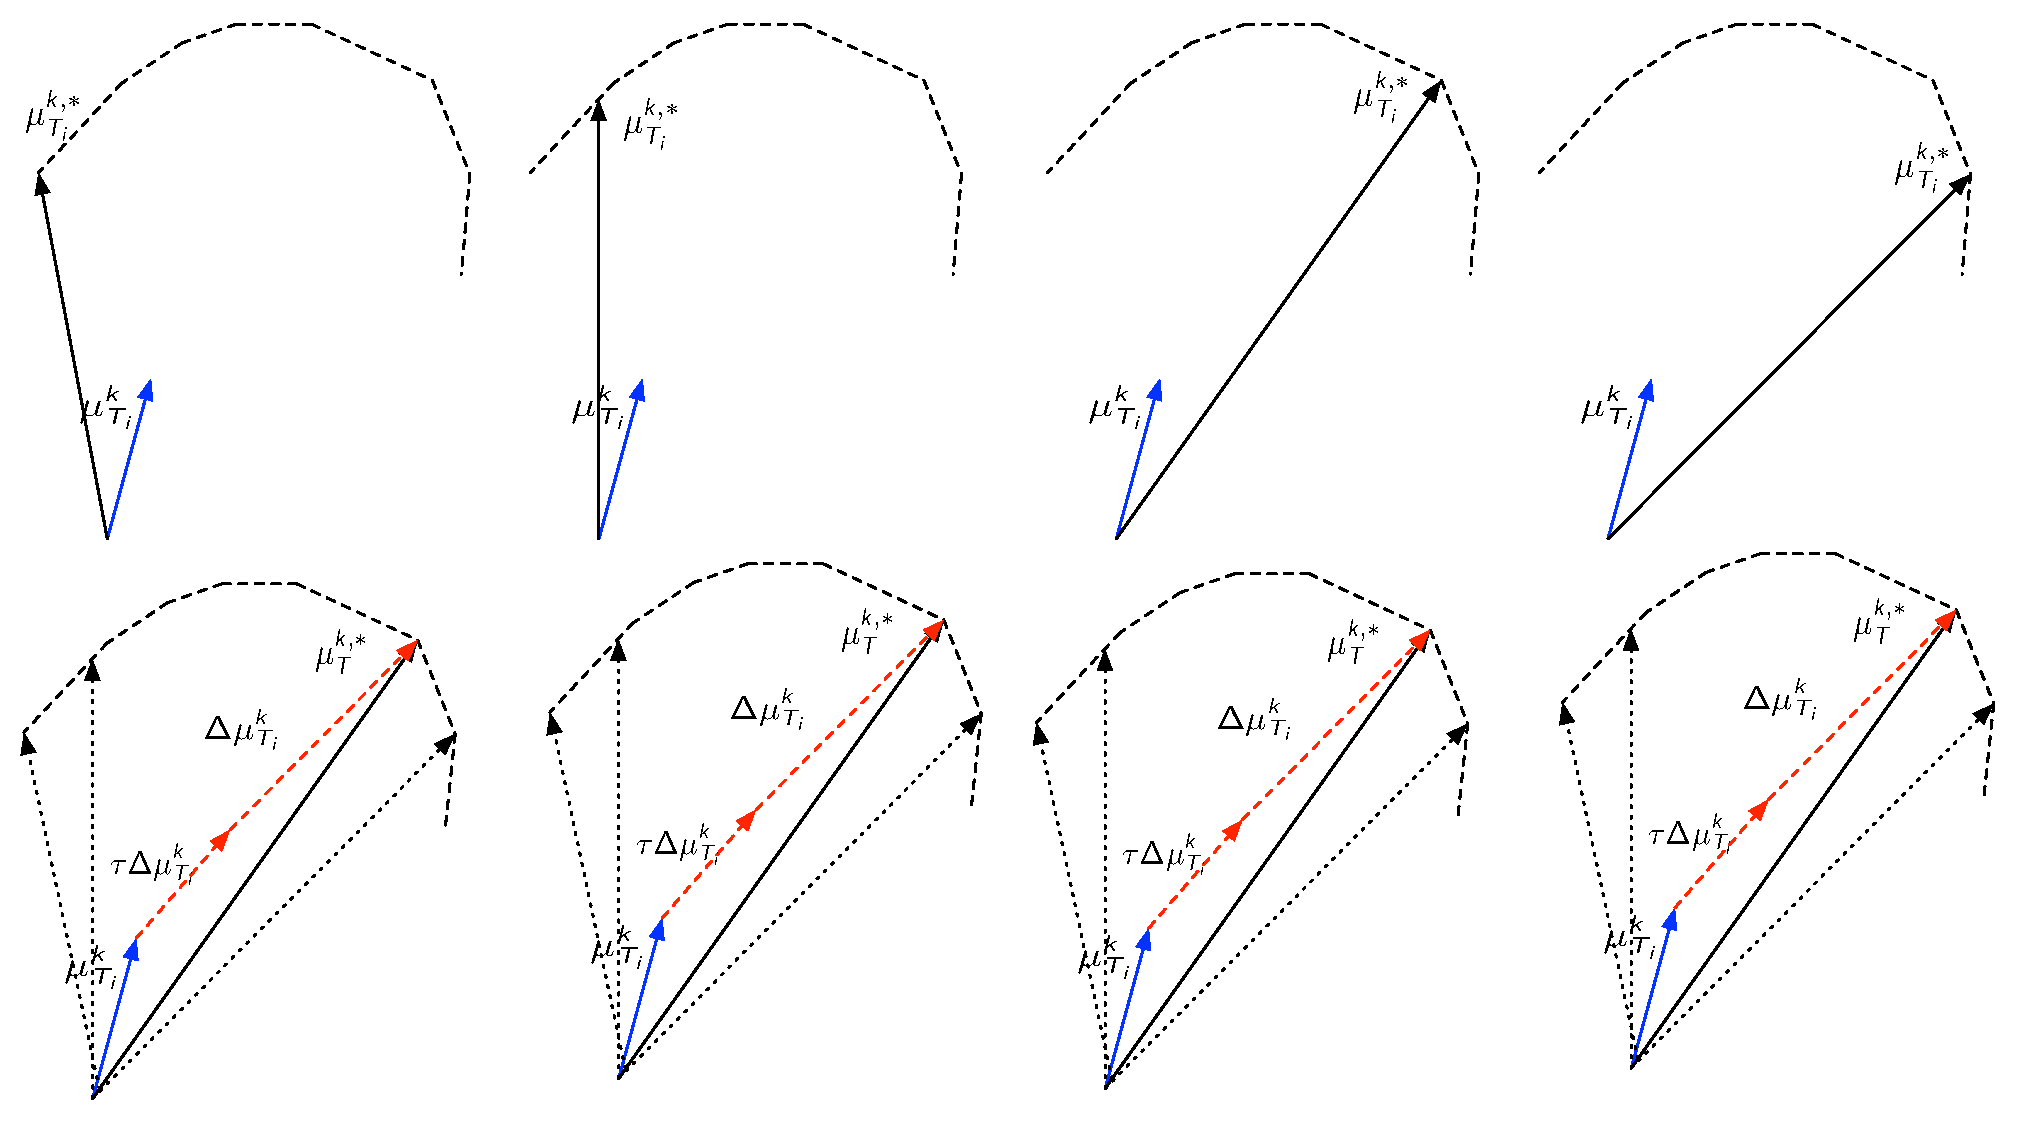
\includegraphics[scale=0.25]{./best_update.pdf}
			\end{center}
		\end{figure}}
		\only<2>
		{\begin{figure}
			\begin{center}
				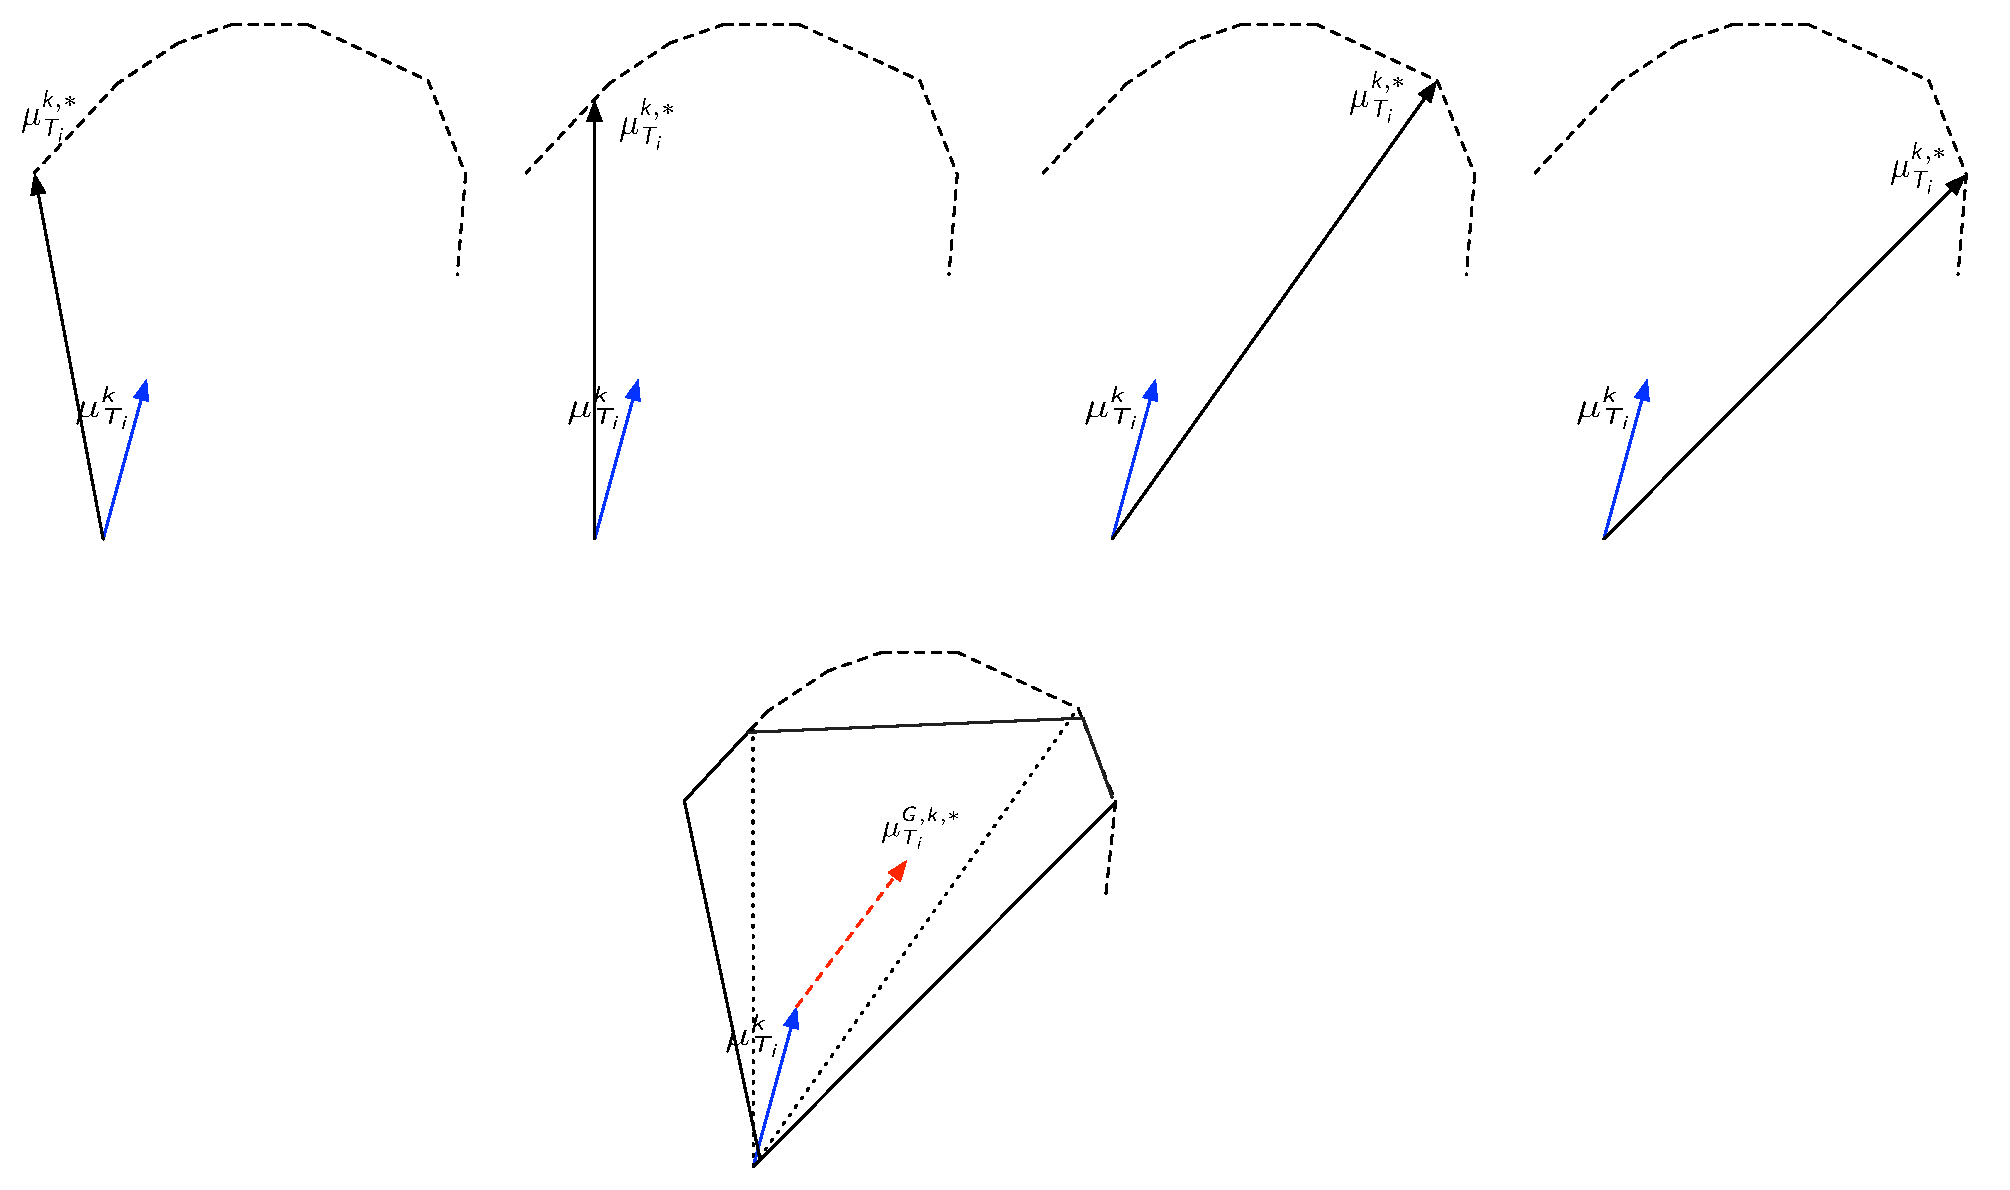
\includegraphics[scale=0.25]{./multiple_update.pdf}
			\end{center}
		\end{figure}}
	\end{itemize}
\end{frame}

%
%
\begin{frame}{Future work}{L$_1$ norm random spanning tree approximation \lonerta}
	\begin{itemize}\footnotesize
		\item From conic combination of a collection of random spanning trees
		\begin{align*}
			F(\vw,\vx,\vy) &= \underset{T\in U(G)}{\E}a_T\ip{\vw_T}{\phib_T(\vx,\vy)}\\
			  &\underset{T\in U(G)}{\E}a_T^2=1,  \underset{T\in U(G)}{\E}a_T<1.
		\end{align*}
		\item To convex combination of a collection of random spanning trees
		\begin{align*}
			F(\vw,\vx,\vy) &= \underset{T\in U(G)}{\E}a_T\ip{\vw_T}{\phib_T(\vx,\vy)}\\
			  &\underset{T\in U(G)}{\E}a_T=1,  \underset{T\in U(G)}{\E}a_T<1.
		\end{align*}
		\item Optimization problem
		\begin{align*}
			\underset{\vw_{T_i},\xi_i}{\minimize} & \quad \frac{1}{2}\left(\sum_{i=1}^{n}\norm{\vw_{T_i}}\right)^2 + C\sum_{k=1}^{m}\xi_k\\
			\st & \quad \frac{1}{{n}}\sum_{i=1}^{n}{ \langle \vw_{T_i}, \phib_{T_t}(\vx_k,\vy_k) \rangle} - \underset{\vy \neq \vy_k}{\maximize\ } \frac{1}{{n}}\sum_{i=1}^{n}{\langle \vw_{T_t}, \phib_{T_i}(\vx_k,\vy) \rangle } \geq 1 -  \xi_k, \\
			& \quad \xi_k\ge0\, , \forall\ k \in \set{1,\dots,m}.
		\end{align*}
	\end{itemize}
\end{frame}






\begin{frame}[allowframebreaks]{Bibliography}
%\bibliographystyle{plain}
\bibliographystyle{apalike}
 \bibliography{dissertation}
\end{frame}

\end{document}
